\documentclass[journal]{IEEEtran}
\usepackage[utf8]{inputenc}
\usepackage[T1]{fontenc}
\usepackage{amsmath,amssymb,amsthm,mathtools}
\usepackage{graphicx}
\usepackage{booktabs}
\usepackage{array}
\usepackage{multirow}
\usepackage{tabularx}
\usepackage{xcolor}
\usepackage{tikz}
\usetikzlibrary{arrows.meta,positioning,shapes.geometric,shapes.symbols,fit,calc,backgrounds,shadows,decorations.pathreplacing}
\usepackage{pgfplots}
\pgfplotsset{compat=1.18}
\usepackage{enumitem}
\usepackage{cite}
\usepackage[hidelinks]{hyperref}
% allow URLs to break at hyphens/slashes in the two-column bibliography
\Urlmuskip=0mu plus 1mu
\expandafter\def\expandafter\UrlBreaks\expandafter{\UrlBreaks
  \do\-\do\_\do\.\do\=\do\?\do\&\do\/\do\a\do\b\do\c\do\d\do\e\do\f
  \do\g\do\h\do\i\do\j\do\k\do\l\do\m\do\n\do\o\do\p\do\q\do\r\do\s
  \do\t\do\u\do\v\do\w\do\x\do\y\do\z\do\0\do\1\do\2\do\3\do\4\do\5
  \do\6\do\7\do\8\do\9}

% ---------- Theorem environments ----------
\newtheorem{theorem}{Theorem}
\newtheorem{proposition}{Proposition}
\newtheorem{corollary}{Corollary}
\newtheorem{lemma}{Lemma}
\newtheorem{definition}{Definition}
\newtheorem{assumption}{Assumption}
\newtheorem{remark}{Remark}

% ---------- Color palette ----------
\definecolor{pxblue}{RGB}{21,67,116}
\definecolor{pxteal}{RGB}{0,128,128}
\definecolor{pxorange}{RGB}{204,102,0}
\definecolor{pxgray}{RGB}{245,246,248}
\definecolor{pxgreen}{RGB}{34,111,60}
\definecolor{pxred}{RGB}{165,42,42}

% ---------- TikZ styles ----------
\tikzset{
  box/.style={draw=pxblue, thick, rounded corners=2pt, fill=pxgray,
    align=center, font=\scriptsize, inner sep=3pt, minimum height=6mm},
  sys/.style={draw=pxblue, thick, rounded corners=2pt, fill=pxblue!8,
    align=center, font=\scriptsize\bfseries, inner sep=3pt, minimum height=7mm},
  newsys/.style={draw=pxorange, thick, rounded corners=2pt, fill=pxorange!10,
    align=center, font=\scriptsize\bfseries, inner sep=3pt, minimum height=7mm},
  ext/.style={draw=pxteal, thick, rounded corners=2pt, fill=pxteal!8,
    align=center, font=\scriptsize, inner sep=3pt, minimum height=6mm},
  node0/.style={draw=pxblue, very thick, fill=pxblue!15, align=center,
    font=\scriptsize\bfseries, inner sep=3pt},
  flow/.style={-{Stealth[length=2mm]}, thick, pxblue},
  flow2/.style={-{Stealth[length=2mm]}, thick, pxteal, dashed},
  flow3/.style={-{Stealth[length=2mm]}, thick, pxorange},
  lbl/.style={font=\tiny, midway, fill=white, inner sep=1pt},
  grp/.style={draw=pxblue!30, fill=pxblue!3, rounded corners=4pt, inner sep=5pt},
  panel/.style={draw=#1!35, fill=#1!4, rounded corners=4pt, inner sep=6pt},
  tab/.style={fill=#1, text=white, font=\tiny\bfseries, rounded corners=2pt,
    inner sep=2.5pt, anchor=south west},
  lane/.style={fill=#1, rounded corners=3pt, draw=none},
  lanetab/.style={fill=#1, text=white, font=\tiny\bfseries, rounded corners=2pt,
    inner sep=2.5pt, anchor=south},
  badge/.style={circle, fill=pxred, text=white, font=\tiny\bfseries,
    inner sep=0.6pt, minimum size=3.2mm},
  chip/.style={draw=#1, fill=#1!10, rounded corners=2pt, font=\tiny,
    inner sep=2pt, minimum height=4mm},
  dim/.style={{Bar[width=1.6mm]}-{Bar[width=1.6mm]}, thin, gray},
}

\begin{document}

\title{ParaExpress: A Mathematically Grounded Hyperlocal Fulfillment Network and Digital Twin Architecture for Instant Beauty Commerce in Indonesia}

\author{ParaTech~Platform~R\&D~Team,~ParagonCorp%
\thanks{Manuscript prepared August 2026. The authors are with the ParaTech Platform Research \& Development Division, PT Paragon Technology and Innovation (ParagonCorp), Jakarta, Indonesia (e-mail: paratech-rnd@paracorpgroup.com).}}

\markboth{ParaTech Platform R\&D Technical Report, Vol.~1, No.~1, August~2026}%
{ParaTech R\&D: ParaExpress Solution Specification}

\maketitle

\begin{abstract}
Instant-delivery platforms such as Shopee Express (SPX~Instant) and Astro now deliver consumer goods within one hour of order placement, and platforms that own the fastest delivery promise increasingly own the consumer relationship---and, eventually, private-label categories that compete with brand manufacturers. This report specifies \emph{ParaExpress}, a brand-owned hyperlocal fulfillment network and digital twin platform that allows ParagonCorp, Indonesia's largest beauty company (16 brands, ${\approx}2{,}000$ SKUs and bundles), to fulfill marketplace and direct orders from the fulfillment node nearest to the consumer within a sub-60-minute service-level agreement (SLA), while preserving the economics of a manufacturer rather than a platform. We (i)~benchmark the fulfillment architectures of Amazon, Alibaba/Cainiao, JD~Logistics, Coupang, and quick-commerce operators; (ii)~formalize the ParaExpress design problem as an SLA-constrained facility-location, inventory-positioning, and order-routing program, and prove structural results---NP-hardness, a $(1-1/e)$ greedy coverage guarantee, unimodality of the network cost in fleet size yielding a unique optimal micro-fulfillment-center (MFC) count, exact greedy optimality of SKU forward-placement under a uniform matroid, and polynomial-time integrality of real-time order routing; (iii)~derive the MFC operating model (location, size, assortment, staffing via square-root safety staffing) from these results; (iv)~specify new capabilities for the existing MagPie, Heron, Exagon, and ShipGo systems plus three new platform services---a Virtual Inventory \& Distributed Order Management service, an Order Routing Engine, and the ParaTwin digital twin; and (v)~define the digital twin's formal state model, calibration data contracts, and experiment portfolio to de-risk the rollout. A partnership topology with marketplaces (Shopee, TikTok Shop/Tokopedia), mid-mile digital 3PLs (e.g., MOSTRANS), and on-demand last-mile fleets (Grab, GoSend) completes an asset-light design in which consignment stores already integrated through Exagon are activated as fulfillment nodes at near-zero incremental fixed cost.
\end{abstract}

\begin{IEEEkeywords}
Distribution network design, e-commerce fulfillment, facility location, digital twin, last-mile logistics, micro-fulfillment center, order management, quick commerce, supply chain optimization, vehicle routing.
\end{IEEEkeywords}

\IEEEpeerreviewmaketitle

\section{Introduction}
\IEEEPARstart{T}{he} economics of consumer commerce in Southeast Asia are being reorganized around the \emph{delivery promise}. Shopee's in-house carrier SPX Express advertises same-day and instant fulfillment in Indonesian metros; quick-commerce operator Astro operates a dense network of dark stores that put a courier at the consumer's door in as little as 15--60 minutes. International precedents---Amazon's regionalized same-day network, Alibaba's Cainiao and Freshippo store-warehouses, JD Logistics' integrated fulfillment estate, and Coupang's density-first Rocket Delivery---demonstrate a consistent endgame: \emph{whoever controls the fastest fulfillment loop accumulates the consumer relationship, the data, and ultimately the shelf}, including private-label brands that displace incumbent manufacturers.

ParagonCorp is Indonesia's largest beauty manufacturer, operating 16 brands (Wardah, Make~Over, Emina, Kahf, Instaperfect, Crystallure, Labor\'e, Biodef, Tavi, Wonderly, Beyondly, OMG, Earth Love Life, Putri, and others) across roughly 2{,}000 active SKUs and bundles. Its current distribution stack---a National Distribution Center (NDC) in Jakarta, a B2C DC in Tegal serving TikTok Shop and Shopee order flow, and a set of B2B DCs (Bogor, Bandung, Solo, Makassar, and others, including Malaysia) serving general- and modern-trade stores---was engineered for \emph{replenishment logistics}: moving cases to stores and parcels to couriers within days. It was not engineered for \emph{instant logistics}: moving a single eyeliner to a consumer in under an hour.

This asymmetry is now strategic. If marketplaces alone can meet the instant promise, ParagonCorp's brands become undifferentiated supply behind someone else's delivery experience. The competitive response specified here is not to out-build Shopee's parcel network, but to \emph{redefine the fulfillment layer for the beauty category}: a hyperlocal, brand-owned network of micro-fulfillment centers (MFCs) and consignment-store fulfillment nodes, fed by the existing NDC/DC backbone via digital mid-mile partners (e.g., MOSTRANS), and delivering through established on-demand fleets (Grab, GoSend) --- so that \emph{any} channel a consumer orders in (Shopee, TikTok Shop/Tokopedia, brand.com, WhatsApp commerce) is fulfilled by the nearest ParagonCorp-controlled node, faster and cheaper per beauty basket than a generalist dark store can achieve.

The contributions of this report are:
\begin{enumerate}[leftmargin=*]
  \item a state-of-the-art benchmark of global and regional instant-fulfillment architectures (Section~\ref{sec:benchmark});
  \item a formal mathematical definition of the ParaExpress network design problem, with theorems and propositions that justify the architecture and make it computable (Sections~\ref{sec:model}--\ref{sec:theory});
  \item the ParaExpress reference network architecture and MFC operating model derived from those results (Sections~\ref{sec:network}--\ref{sec:fc});
  \item the business model and partnership topology (Section~\ref{sec:business});
  \item the solution specification: new features for MagPie, Heron, Exagon, and ShipGo, and the new Virtual Inventory/DOM, Order Routing Engine, and ParaTwin systems (Section~\ref{sec:systems});
  \item the ParaTwin digital twin formal model, data contracts, and experiment plan for 16 brands and ${\approx}2{,}000$ SKUs (Section~\ref{sec:twin});
  \item a phased implementation roadmap with pilot acceptance criteria (Section~\ref{sec:roadmap}).
\end{enumerate}

\section{State-of-the-Art Benchmark}
\label{sec:benchmark}
We benchmark the fulfillment architectures that define the global and regional state of the art, then extract the design lessons that ParaExpress adopts or deliberately inverts. Table~\ref{tab:benchmark} summarizes.

\subsection{Amazon: Regionalization and Sub-Same-Day Sites}
Amazon's United States network is a multi-echelon hierarchy of inbound cross-docks, fulfillment centers (FCs), sortation centers, and delivery stations---more than 600 logistics sites \cite{redstag}. Two recent moves matter most for ParaExpress. First, the 2023 \emph{regionalization} partitioned the national network into eight largely self-sufficient regions with fast-moving inventory replicated in each; in-region fulfillment rose from 62\% to 76\% of ordered products, and 2023 cost-to-serve fell by more than \$0.45 per unit---the first reduction since 2018---while over 7 billion items were delivered same- or next-day \cite{amazonregional,scdive,amazonscience}. Second, Amazon's \emph{sub-same-day} (SSD) sites---facilities roughly one-tenth the size of a classical FC that collapse FC, sortation, and delivery station under one roof---achieve an average pick-to-outbound-dock time of 11 minutes and anchor the same-day promise in the top metros, where about 60\% of Prime orders now arrive same- or next-day \cite{costar,cnbcprime}. Amazon's anticipatory-shipping patent formalizes the underlying doctrine: move inventory toward predicted demand \emph{before} the order exists \cite{anticipatory}. Robotics (the million-robot fleet, Sequoia stowing) compresses in-node time \cite{sequoia,millionrobot}.

\subsection{Alibaba/Cainiao and the Freshippo Store-as-Warehouse}
Cainiao orchestrates a largely partner-operated network (${\sim}$170--200 warehouses, 170{,}000+ neighborhood pickup points) through a data layer---the standardized electronic waybill---rather than through asset ownership, and offers half-day/same-day products in ${\sim}$300 cities \cite{cainiao,cainiaoexpress}. The most transferable pattern for ParagonCorp is Freshippo (Hema): each store doubles as a fulfillment node with in-aisle picking, overhead-conveyor consolidation, and a 30-minute promise within a 3~km radius; about 60\% of store throughput is online orders \cite{hema}. Freshippo proves that \emph{existing retail assets can be converted into an instant-fulfillment network} when picking and inventory accuracy are engineered deliberately---precisely the ParaExpress consignment-store thesis.

\subsection{JD Logistics: Front Distribution Centers}
JD holds first-party inventory deep in the network---800+ warehouses organized as 8 large regional distribution centers (RDCs) feeding small, district-level \emph{front distribution centers} (FDCs) stocked with local fast movers---and delivers ${\sim}$90\% of orders same- or next-day \cite{jdwarehouses}. JD's deployed assortment-planning and inventory-allocation system (forecasting + optimization + simulation over all eight RDCs) reports savings of \${}6.1M/yr in holding cost and \${}22.3M/yr in transfer cost with a $+0.85$~pp availability gain \cite{jdassort}---direct evidence that the forward-assortment problem $(\mathsf{P2})$ and its digital-twin evaluation loop are where the money is.

\subsection{Coupang: Density as Strategy}
Coupang's Rocket Delivery guarantees next-day (and dawn) delivery on millions of SKUs; the structural fact is density---70\% of South Koreans live within ${\sim}$11~km of a Coupang fulfillment center, across 100+ facilities and 55M+ sq~ft built with ${\sim}$\$4.6B of cumulative logistics investment \cite{coupang,coupanginnov}. Coupang demonstrates the endgame ParagonCorp must respect: once a platform achieves fulfillment density, it converts speed into membership lock-in (14M Rocket WOW members, nearly one in four Koreans).

\subsection{Quick Commerce: Failures Abroad, Proof in India}
The 2021--2024 dark-store wave supplies both the template and the cautionary tale. The template: 200--700~m$^2$ dark stores, 1{,}000--3{,}500 SKUs, 1.5--3~km radius, 10--30-minute promises; delivery-cycle anatomy of 2--3~min pick, ${\sim}$1~min rider assignment, 5--6~min transit \cite{qcops,blinkit}. The cautionary tale: Getir fell from an \$11.8B valuation to a retreat from all Western markets in April 2024, after promotion-fueled growth with sub-scale order density and low AOV \cite{getir,sifted}. The proof: India's Blinkit (1{,}800+ dark stores) and Zepto turned the same template contribution-margin positive via order density, AOV discipline, and disciplined assortment \cite{indiaqc,blinkit}. The ParaExpress inference is category-structural: beauty baskets carry 2--4$\times$ grocery AOV, zero cold chain, and high value density, so the \emph{same} dark-store mechanics clear break-even at a fraction of grocery's required order density (Table~\ref{tab:econ}).

\subsection{Store-Based Fulfillment: Walmart and Target}
Walmart reaches 93\% of US households with same-day delivery from ${\sim}$3{,}900 stores; store-fulfilled delivery sales tripled in two years to over \$1B/month \cite{walmart,walmartsales}. Target fulfills 95\%+ of total orders from stores, using sortation centers and the Shipt fleet for next-day density \cite{target}. Both trade warehouse pick efficiency for near-zero incremental real estate and radically shorter last miles---the exact trade Corollary~\ref{cor:stores} formalizes for ParagonCorp's consignment estate.

\subsection{The Indonesian Battlefield}
Shopee holds ${\sim}$46\% of Indonesian e-commerce GMV and a dominant ${\sim}$63\% share of platform beauty GMV \cite{shopeeshare,shopeebeauty}; its carrier SPX Express covers 514 cities/regencies, and in February 2025 Shopee deployed 200 micro-fulfillment centers in tier-2/3 cities (a US\$120M program targeting ${\sim}$40\% faster delivery) \cite{spx,shopeemfc}. TikTok Shop/Tokopedia reached ${\sim}$US\$13B Indonesian GMV in 2025 \cite{tiktok,tiktokgmv}. Astro operates ${\sim}$50 dark stores in Jabodetabek with ${\sim}$1{,}500 hyperlocalized SKUs, 2--3~km radii, and 15-minute delivery \cite{astrotc,astroken,astrogpca}. On-demand last-mile capacity is commoditized and API-accessible: GrabExpress Instant (pickup ${\sim}$30~min, distance-based per-km pricing) and GoSend Instant (max 40~km, 20~kg, lifecycle webhooks) both expose merchant APIs \cite{grab,gosend}. Mid-mile digital 3PL capacity exists in MOSTRANS (Kalbe/Enseval group): 70+ transporters, 5{,}000+ GPS-equipped trucks, ambient/cool/cold chain, e-POD, and ERP integration \cite{mostrans,mostranskalbe}. Indonesian quick commerce is projected to grow from ${\sim}$US\$1.4--3.1B (2025, definitions vary) at 6--8\% CAGR, with minimarket chains (Alfamart ${\sim}$50 dark stores) entering O2O fulfillment \cite{qcmarket}---evidence that the instant tier is becoming table stakes, not a niche.

\subsection{Design Lessons Adopted by ParaExpress}
\begin{enumerate}[leftmargin=*, label=\textbf{L\arabic*.}]
  \item \emph{Regionalize inventory} ahead of demand; measure in-region fulfillment share as a first-class KPI (Amazon) \cite{amazonregional}.
  \item \emph{Collapse echelons for speed}: the instant tier needs single-roof pick-to-courier in ${\le}$11--15 min, not a chain of touches (Amazon SSD, Blinkit) \cite{costar,blinkit}.
  \item \emph{Convert existing retail into fulfillment}: engineered in-store picking with a hard promise radius (Freshippo, Walmart, Target) \cite{hema,walmart,target}.
  \item \emph{Solve assortment + allocation with a simulation loop}, not spreadsheets (JD) \cite{jdassort}.
  \item \emph{Density before geography}: saturate one metro to SLA-profitability before replicating (Coupang; Getir's inverse) \cite{coupang,getir}.
  \item \emph{Respect unit economics}: AOV discipline and order density decide survival; beauty's category economics are structurally favorable (India QC) \cite{indiaqc}.
  \item \emph{Own the data plane, rent the assets}: electronic-waybill-style standardization over partner fleets (Cainiao; MOSTRANS/Grab for ParagonCorp) \cite{cainiao,mostrans}.
  \item \emph{The promise is computed, not configured}: dynamic, honest delivery promises shown pre-checkout drive conversion (all benchmarks).
\end{enumerate}

\begin{table*}[!t]
\caption{State-of-the-Art Benchmark of Instant/Fast Fulfillment Architectures (compiled Aug.\ 2026)}
\label{tab:benchmark}
\centering
\scriptsize
\begin{tabularx}{\textwidth}{@{}p{20mm} p{28mm} p{28mm} p{22mm} p{22mm} X@{}}
\toprule
\textbf{Operator} & \textbf{Model} & \textbf{Node scale} & \textbf{Assortment/node} & \textbf{Promise} & \textbf{Key mechanism} \\
\midrule
Amazon \cite{amazonregional,costar} & Regionalized FC + SSD sites & 600+ sites; SSD ${\sim}$10\% of FC size & FC: wide; SSD: fast movers & Same/next day; ${\sim}$5 h SSD & 8 self-sufficient regions; 11-min pick-to-dock; anticipatory placement \\
Cainiao/Freshippo \cite{cainiao,hema} & Data-plane 3PL + store-as-warehouse & ${\sim}$200 warehouses; stores 3 km radius & Store: full range & Half-day; 30 min (Hema) & E-waybill data standard; in-aisle pick + conveyor consolidation \\
JD Logistics \cite{jdwarehouses,jdassort} & Owned RDC$\to$FDC hierarchy & 800+ warehouses; 8 RDCs & FDC: local fast movers & ${\sim}$90\% same/next day & Deep first-party inventory; ML assortment + allocation + simulation \\
Coupang \cite{coupang} & Density-first owned network & 100+ centers, 55M+ sq ft & Wide & Next day / dawn & 70\% of population within ${\sim}$11 km; membership flywheel \\
Blinkit/Zepto \cite{indiaqc,blinkit} & Dark stores & 1{,}100--1{,}800 stores & 1--3.5k SKUs & 10--20 min & 2--3 min pick; 1.5--3 km radius; AOV discipline \\
Walmart/Target \cite{walmart,target} & Ship-from-store & 3{,}900+ stores (WMT) & Store range & Same day & Store estate as forward network; sortation for density \\
SPX/Shopee \cite{spx,shopeemfc} & Marketplace carrier + MFCs & 514 cities; 200 MFCs (2025) & Marketplace-wide & Same day/instant (metros) & Captive parcel network; tier-2/3 MFC push \\
Astro \cite{astroken,astrogpca} & Pure dark-store q-commerce & ${\sim}$50 stores (Jabodetabek) & ${\sim}$1{,}500 SKUs & ${\sim}$15--60 min & Hyperlocal assortment per store; 2--3 km radius \\
\midrule
\textbf{ParaExpress (this work)} & \textbf{Brand-owned hybrid: store nodes + dark MFCs} & \textbf{per-metro $\max(n_{\min}, n^\star)$ (Thm.~\ref{thm:ncost})} & \textbf{150--1{,}200 SKUs (Thm.~\ref{thm:assortment})} & \textbf{$\le$60 min @ 95\% ($\mathsf{PX1}$)} & \textbf{Channel-agnostic routing (Thm.~\ref{thm:routing}); consignment estate as zero-capex coverage; rented mid/last mile} \\
\bottomrule
\end{tabularx}
\end{table*}

\section{Formal Problem Definition}
\label{sec:model}
We now give a formal definition of the ParaExpress design problem. The formulation is deliberately layered: a \emph{strategic} layer (where to open fulfillment nodes and what to stock), a \emph{tactical} layer (replenishment and staffing), and an \emph{operational} layer (real-time order routing and dispatch). Each layer is an optimization problem whose structure we exploit in Section~\ref{sec:theory}, and each is mirrored one-to-one by a module of the ParaTwin digital twin (Section~\ref{sec:twin}).

\subsection{Network, Demand, and SLA Primitives}

\begin{definition}[Fulfillment graph]
\label{def:graph}
The ParaExpress network is a directed graph $G=(\mathcal{N},\mathcal{A})$ whose node set
$\mathcal{N} = \{0\} \cup \mathcal{D} \cup \mathcal{F} \cup \mathcal{Z}$
comprises the NDC (node $0$), the set of regional DCs $\mathcal{D}$ (B2C~DC Tegal and B2B DCs), the set of \emph{candidate fulfillment nodes} $\mathcal{F} = \mathcal{F}^{\mathrm{mfc}} \cup \mathcal{F}^{\mathrm{store}}$ (own micro-fulfillment centers and Exagon consignment stores), and the set of demand zones $\mathcal{Z}$ (e.g., kelurahan-level polygons). Arcs $\mathcal{A}$ carry mid-mile flows ($0 \to \mathcal{D} \to \mathcal{F}$) and last-mile flows ($\mathcal{F} \to \mathcal{Z}$).
\end{definition}

\begin{definition}[Demand field]
\label{def:demand}
Let $\mathcal{K}$ denote the SKU catalog, $|\mathcal{K}| \approx 2{,}000$ across 16 brands. Instant-channel demand in zone $z \in \mathcal{Z}$ for SKU $k \in \mathcal{K}$ is a marked Poisson process with rate $\lambda_{zk} \geq 0$ orders per hour; $\lambda_z = \sum_k \lambda_{zk}$ and $\Lambda = \sum_z \lambda_z$. Order composition (basket of SKUs and bundle explosions) follows a distribution $\mathcal{B}_z$ estimated from MagPie history.
\end{definition}

\begin{definition}[Service promise]
\label{def:sla}
A \emph{promise class} is a pair $(\tau, \alpha)$: the order must be delivered within $\tau$ minutes of payment with probability at least $\alpha$. ParaExpress operates three classes:
$\mathsf{PX1} = (60\,\text{min}, 0.95)$ (instant), $\mathsf{PX2} = (240\,\text{min}, 0.95)$ (same-day slot), and $\mathsf{PX3}$ (next-day, fulfilled by the existing Tegal B2C DC flow). The end-to-end sojourn of an order decomposes as
\begin{equation}
\label{eq:sojourn}
T = T_{\mathrm{route}} + T_{\mathrm{queue}} + T_{\mathrm{pick}} + T_{\mathrm{handover}} + T_{\mathrm{travel}},
\end{equation}
i.e., routing decision, waiting for a picker, pick--pack, courier pickup, and travel to the consumer.
\end{definition}

\subsection{Strategic Layer: SLA-Constrained Location--Allocation}

Binary variables $y_f \in \{0,1\}$ open node $f\in\mathcal{F}$ (for a consignment store, ``opening'' means activating it as a fulfillment node with dedicated ParaExpress stock and app tooling); $x_{fz} \in [0,1]$ is the fraction of zone $z$'s instant demand assigned to $f$. Let $t_{fz}$ be the $\alpha$-quantile of $T$ in \eqref{eq:sojourn} when $f$ serves $z$ (travel times from the road network / Grab historical data), and let the \emph{coverage set} be $\mathcal{F}(z) = \{f : t_{fz} \le \tau\}$. With fixed cost $c^{\mathrm{fix}}_f$ per period (rent, staff, equipment amortization; near-zero for store nodes), variable fulfillment cost $c^{\mathrm{var}}_{fz}$ per order (pick, pack, courier fee $f\!\to\!z$), and per-order gross margin $m$, the strategic problem is:
\begin{align}
(\mathsf{P1})\quad \max_{x,y}\ & \sum_{z\in\mathcal{Z}} \sum_{f \in \mathcal{F}(z)} \big(m - c^{\mathrm{var}}_{fz}\big)\, \lambda_z\, x_{fz} - \sum_{f\in\mathcal{F}} c^{\mathrm{fix}}_f\, y_f \label{eq:p1obj}\\
\text{s.t. } & \textstyle\sum_{f \in \mathcal{F}(z)} x_{fz} \le 1, \quad \forall z \in \mathcal{Z}, \label{eq:p1assign}\\
& x_{fz} \le y_f, \quad \forall f, z, \label{eq:p1open}\\
& \textstyle\sum_{z} \lambda_z x_{fz} \le \mu_f\, y_f, \quad \forall f \in \mathcal{F}, \label{eq:p1cap}\\
& x_{fz} \ge 0,\ y_f \in \{0,1\}, \nonumber
\end{align}
where $\mu_f$ is node $f$'s sustainable throughput (orders/hour) from its staffing and layout (Section~\ref{sec:fc}). Constraint~\eqref{eq:p1assign} allows demand to remain unserved by $\mathsf{PX1}$ (it falls back to $\mathsf{PX2}/\mathsf{PX3}$), \eqref{eq:p1open} links assignment to opening, and \eqref{eq:p1cap} enforces throughput. $(\mathsf{P1})$ generalizes the capacitated facility-location problem \cite{daskin,melo} with an SLA-induced coverage structure \cite{church}.

\subsection{Strategic Layer: Forward Assortment (What to Stock Where)}

An MFC cannot hold 2{,}000 SKUs; it holds a forward assortment $S_f \subseteq \mathcal{K}$ limited by shelf capacity $V_f$ (slots). Let $w_k$ be the slot requirement of SKU $k$ and $r_{fk}$ the instant-demand revenue rate captured if $k$ is stocked at $f$ (orders containing an unstocked SKU either split, downgrade to $\mathsf{PX2}$, or are lost with probability $\theta$). The assortment problem at node $f$ is
\begin{equation}
\label{eq:assort}
(\mathsf{P2})\quad \max_{S \subseteq \mathcal{K}} \ \sum_{k \in S} r_{fk} \quad \text{s.t.} \quad \sum_{k \in S} w_k \le V_f .
\end{equation}
With basket effects, the objective generalizes to $R_f(S) = \mathbb{E}_{\mathcal{B}}[\,m(B)\,\mathbf{1}\{B \subseteq S\}\,]$ over baskets $B$, which is monotone but not modular; Section~\ref{sec:theory} gives exact and approximate solutions for the practically relevant cases.

\subsection{Tactical Layer: Inventory Positioning and Replenishment}

Each stocked SKU $k$ at node $f$ follows a periodic base-stock policy with review period $T_r$ (replenishment wave from the parent DC via mid-mile), lead time $L_f$, and base-stock level
\begin{equation}
\label{eq:basestock}
b_{fk} = \underbrace{\lambda_{fk} (T_r + L_f)}_{\text{cycle stock}} + \underbrace{z_{\beta}\, \sigma_{fk} \sqrt{T_r + L_f}}_{\text{safety stock}},
\end{equation}
where $\lambda_{fk}, \sigma_{fk}$ are the mean and standard deviation \emph{per unit time} of demand allocated to $f$ (so safety stock scales with $\sqrt{T_r + L_f}$ under independent increments), $z_\beta = \Phi^{-1}(\beta)$, and $\beta$ is the in-node fill-rate target (newsvendor critical fractile \cite{eppen,graves}). Replenishment quantities feed a mid-mile vehicle-routing problem over $\mathcal{D} \to \mathcal{F}$ executed by the 3PL (MOSTRANS), a capacitated VRP with time windows \cite{tothvigo}.

\subsection{Operational Layer: Real-Time Order Routing}

At decision epoch $t$, let $O(t)$ be the set of open instant orders and for order $o$ let $\mathcal{F}(o) \subseteq \mathcal{F}$ be the nodes that (i)~cover $o$'s zone within the promise, (ii)~have all SKUs of $o$'s basket in available-to-promise (ATP) virtual inventory, and (iii)~have residual picking capacity. With routing cost $c_{of}$ (courier fee + marginal congestion cost + inventory-displacement penalty), the router solves
\begin{equation}
\label{eq:p3}
\begin{split}
(\mathsf{P3})\quad \min_{u}\ & \sum_{o \in O(t)} \sum_{f \in \mathcal{F}(o)} c_{of}\, u_{of} \\
\text{s.t.}\ & \textstyle\sum_{f} u_{of} = 1 \ \ \forall o, \qquad \textstyle\sum_{o} u_{of} \le \kappa_f(t) \ \ \forall f,
\end{split}
\end{equation}
with $u_{of} \in \{0,1\}$ and $\kappa_f(t)$ the remaining slot capacity of $f$ in the current wave. $(\mathsf{P3})$ is re-solved every few seconds (or on each order arrival) by the Order Routing Engine; Theorem~\ref{thm:routing} shows it is exactly solvable in real time.

\subsection{Operational Layer: In-Node Queueing and Dispatch}

Node $f$ with $c_f$ pickers is modeled as an $M/M/c_f$ queue with arrival rate $\lambda_f = \sum_z \lambda_z x_{fz}$ and pick--pack rate $\nu$ per picker; courier arrival after handover request is an independent delay $D^{\mathrm{grab}}_f$ (empirically log-normal from Grab/GoSend APIs). The $\mathsf{PX1}$ promise requires
\begin{equation}
\label{eq:slaqueue}
\Pr\!\big[T_{\mathrm{queue}} + T_{\mathrm{pick}} + T_{\mathrm{handover}} + T_{\mathrm{travel}} \le \tau - T_{\mathrm{route}}\big] \ge \alpha,
\end{equation}
which couples staffing $c_f$ to demand (Proposition~\ref{prop:staffing}) \cite{halfin,dekoster}.

\section{Structural Results}
\label{sec:theory}
The formulations above are not merely descriptive; their mathematical structure dictates the ParaExpress architecture. This section states the results and their design consequences. Proofs are given inline when short and sketched otherwise.

\subsection{Hardness and Why a Digital Twin Is Necessary}

\begin{theorem}[NP-hardness of network design]
\label{thm:nphard}
Problem $(\mathsf{P1})$ is NP-hard, even with uncapacitated nodes, uniform margins, and a single SKU.
\end{theorem}
\begin{IEEEproof}
Take an instance of \textsc{Set Cover} with universe $U$ and family $\mathcal{S}$. Build one demand zone per element $u \in U$ with $\lambda_z = 1$ and one candidate node per set $S \in \mathcal{S}$ with $t_{fz} \le \tau$ iff $u \in S$, $c^{\mathrm{fix}}_f = \varepsilon$, $\mu_f = \infty$, and $m - c^{\mathrm{var}}_{fz} = M \gg |\mathcal{S}|\varepsilon$. Any optimal solution of $(\mathsf{P1})$ covers all zones (each unit of covered demand is worth $M$), and among covering solutions maximizing \eqref{eq:p1obj} is equivalent to minimizing $\sum_f y_f$; hence an optimal $(\mathsf{P1})$ solution yields a minimum set cover. \textsc{Set Cover} is NP-hard \cite{gareyjohnson}, so $(\mathsf{P1})$ is NP-hard.
\end{IEEEproof}

\begin{remark}
Theorem~\ref{thm:nphard} is the formal justification for the ParaTwin program: the strategic design space cannot be searched exactly at national scale, so ParaExpress pairs (i)~approximation algorithms with provable guarantees for candidate generation with (ii)~high-fidelity digital twin simulation for candidate evaluation, rather than trusting a single monolithic MILP solve.
\end{remark}

\subsection{Coverage Is Submodular: Greedy Rollout Is Near-Optimal}

Let $g(Y)$ denote the optimal value of \eqref{eq:p1obj} restricted to open set $Y \subseteq \mathcal{F}$ with the fixed-cost term removed, i.e., the maximum SLA-covered contribution achievable with nodes $Y$.

\begin{theorem}[Near-optimal greedy expansion]
\label{thm:submodular}
In the uncapacitated case ($\mu_f = \infty$), $g$ is monotone nondecreasing and submodular:
$g(Y \cup \{f\}) - g(Y) \ge g(Y' \cup \{f\}) - g(Y')$ for all $Y \subseteq Y' \subseteq \mathcal{F}$, $f \notin Y'$.
Consequently, for any budget of $p$ nodes, the greedy algorithm that repeatedly opens the node with the largest marginal covered contribution attains at least $(1 - 1/e) \approx 63.2\%$ of the optimal covered contribution, and this is the best possible guarantee for any polynomial algorithm unless $\mathrm{P}=\mathrm{NP}$.
\end{theorem}
\begin{IEEEproof}
With $\mu_f = \infty$, each zone is served entirely by its best open covering node, so
$g(Y) = \sum_z \lambda_z \max_{f \in Y \cap \mathcal{F}(z)} (m - c^{\mathrm{var}}_{fz})^+$ (with $\max_\emptyset = 0$). Each summand is a maximum of nonnegative node-values over the chosen set, which is monotone and submodular; nonnegative sums preserve both properties. The $(1-1/e)$ guarantee for greedy maximization of a monotone submodular function under a cardinality constraint is the classical result of Nemhauser, Wolsey, and Fisher \cite{nemhauser}, applied to floor-space location by Cornuejols~et~al.~\cite{cornuejols}; the matching inapproximability bound is Feige's \cite{feige}.
\end{IEEEproof}

\begin{corollary}[Consignment stores strictly dominate as first waves]
\label{cor:stores}
Because $g$ is monotone, activating an Exagon consignment store as a fulfillment node never reduces covered contribution, and since $c^{\mathrm{fix}}_f \approx 0$ for such nodes, any store with positive marginal coverage improves profit. Diminishing returns (submodularity) imply the correct rollout order is by \emph{marginal} coverage, recomputed after each activation---not by store size or standalone sales.
\end{corollary}

Corollary~\ref{cor:stores} is the mathematical core of the ParaExpress asset-light thesis: the consignment estate already integrated in Exagon is a zero-capex coverage endowment that competitors without a store network cannot replicate.

\subsection{How Many Nodes: Risk Pooling vs.\ Proximity}

Opening more nodes shortens the last mile but fragments inventory. The trade-off admits a clean characterization under a continuous approximation \cite{daganzo,eppen}.

\begin{assumption}
\label{ass:continuum}
A metro of area $A$ with uniform instant demand density $\rho$ (orders/hr/km$^2$, $\Lambda = \rho A$) is served by $n$ identical nodes with balanced catchments; couriers travel at effective speed $v$; per-node fixed cost rate is $F$; holding cost rate per unit of safety stock is $h$; aggregate demand volatility over the replenishment horizon is $\sigma$ (units).
\end{assumption}

\begin{lemma}[Continuous approximation of the last mile]
\label{lem:ca}
Under Assumption~\ref{ass:continuum}, the expected courier travel distance per order is $d(n) = k \sqrt{A/n}$ for a constant $k$ depending on the metric and catchment shape ($k \approx 0.38$ for Euclidean travel to a centrally located depot in a compact catchment; higher for grid metrics) \cite{daganzo}.
\end{lemma}

\begin{proposition}[Square-root inventory penalty]
\label{prop:pooling}
If metro demand is split evenly across $n$ nodes with independent zone demands, the total safety stock required for a common fill rate $\beta$ is $z_\beta \sigma \sqrt{n}$, i.e., decentralization inflates safety stock by $\sqrt{n}$ relative to a single pooled node \cite{eppen}.
\end{proposition}
\begin{IEEEproof}
Each node faces demand std.\ dev.\ $\sigma/\sqrt{n}$ (independent splitting), holds $z_\beta \sigma / \sqrt{n}$, and there are $n$ nodes.
\end{IEEEproof}

\begin{theorem}[Unique optimal node count]
\label{thm:ncost}
Let the system cost rate be
\begin{equation}
\label{eq:cn}
C(n) = F n + a \sqrt{n} + b\, n^{-1/2},\ \ a = h z_\beta \sigma,\ \ b = \Lambda c_d k \sqrt{A},
\end{equation}
where $c_d$ is courier cost per km. Then $C$ is strictly unimodal on $(0,\infty)$ with a unique minimizer $n^\star$, the unique positive root of $F n^{3/2} + \tfrac{a}{2} n - \tfrac{b}{2} = 0$; equivalently $x = \sqrt{n^\star}$ solves the cubic $2F x^{3} + a x^{2} - b = 0$. In the asset-light regime $F \to 0$ (consignment nodes), $n^\star \to b/a = \Lambda c_d k \sqrt{A} \,/\, h z_\beta \sigma$, i.e., the optimal node count scales \emph{linearly} with delivered volume $\Lambda$ and inversely with volatility $\sigma$.
\end{theorem}
\begin{IEEEproof}
$C'(n) = F + \tfrac{a}{2} n^{-1/2} - \tfrac{b}{2} n^{-3/2}$. Multiplying by $n^{3/2} > 0$ gives $\psi(n) = F n^{3/2} + \tfrac{a}{2} n - \tfrac{b}{2}$, which is strictly increasing with $\psi(0^+) = -b/2 < 0$ and $\psi(\infty) = \infty$; hence $C' < 0$ before the unique root $n^\star$ of $\psi$ and $C' > 0$ after, establishing unimodality and uniqueness. Setting $F=0$ reduces $\psi$ to $\tfrac{a}{2} n - \tfrac{b}{2}$, giving $n^\star = b/a$.
\end{IEEEproof}

\begin{remark}[Numerical validation]
\label{rem:numcheck}
All closed forms in this section are cross-checked in ParaTwin against brute-force evaluation. For the illustrative parameters of Fig.~\ref{fig:costcurve} $(F,a,b) = (1.2, 6, 120)$, the cubic $2.4x^3 + 6x^2 - 120 = 0$ has its unique positive root at $x \approx 3.008$, hence $n^\star \approx 9.1$ and $C(n^\star) \approx 68.8$---matching the plotted minimum. The $F=0$ formula gives $b/a = 20$, correctly larger: removing fixed cost always (weakly) increases the optimal node count since $\psi$ shifts down.
\end{remark}

\begin{proposition}[SLA feasibility floor]
\label{prop:floor}
Fix promise $(\tau,\alpha)$ and let $t^{\alpha}_{\mathrm{node}}$ be the $\alpha$-quantile of in-node time ($T_{\mathrm{queue}}+T_{\mathrm{pick}}+T_{\mathrm{handover}}$). The feasible service radius is $R = v\,(\tau - T_{\mathrm{route}} - t^{\alpha}_{\mathrm{node}})^{+}$ and any design covering area $A$ requires
\begin{equation}
\label{eq:floor}
n \ \ge\ n_{\min} = \Big\lceil \frac{A}{\eta\, \pi R^{2}} \Big\rceil,
\end{equation}
where $\eta \le 1$ is the effective packing/overlap efficiency of catchments on the road network. The binding node count is $\max(n_{\min}, n^\star)$; if $n_{\min} > n^\star$, the SLA---not cost---sizes the network, and every reduction of in-node time $t^{\alpha}_{\mathrm{node}}$ (better picking, faster courier matching) increases $R$ and reduces the required node count \emph{quadratically}.
\end{proposition}

Proposition~\ref{prop:floor} quantifies why ParaExpress invests in pick--pack speed and courier pre-matching (Section~\ref{sec:systems}): a 3-minute reduction of in-node time at $v = 20$ km/h widens the radius by 1~km, which at typical Jakarta densities removes whole nodes from the requirement.

\subsection{Assortment: Exact Greedy Under Uniform Slots}

\begin{theorem}[Forward assortment]
\label{thm:assortment}
(i)~If all SKUs consume equal slots ($w_k \equiv 1$), $(\mathsf{P2})$ is a maximization over a uniform matroid and the greedy rule---stock the $V_f$ SKUs with the highest captured revenue rate $r_{fk}$---is \emph{exactly optimal}.
(ii)~For general $w_k$, $(\mathsf{P2})$ is a 0--1 knapsack: NP-hard but admits an FPTAS, and density-greedy (rank by $r_{fk}/w_k$, take the better of the greedy prefix and the single best item) is a $\tfrac12$-approximation \cite{knapsack}.
(iii)~With basket-completeness objective $R_f(S)$ optimized over brand blocks (bundles and regimen sets never split across the block boundary), the block-level problem is monotone submodular maximization under a knapsack constraint; partial-enumeration greedy attains $(1-1/e)$ \cite{sviridenko}, and if baskets are single-brand with probability $\ge 1 - \epsilon$ (empirically high in beauty), the guarantee on full basket revenue degrades by at most the factor $(1-\epsilon)$.
\end{theorem}
\begin{IEEEproof}[Proof sketch]
(i)~Uniform-matroid greedy optimality is elementary (exchange argument). (ii)~Standard knapsack results \cite{knapsack}. (iii)~Block-restricted $R_f$ is a nonnegative weighted coverage function over disjoint blocks, hence monotone submodular; Sviridenko's algorithm gives $(1-1/e)$ under the slot-budget knapsack \cite{sviridenko}, and cross-brand baskets, which occur with probability $\le \epsilon$, bound the unmodeled revenue.
\end{IEEEproof}

Theorem~\ref{thm:assortment} justifies the operating rule of Section~\ref{sec:fc}: a 400--600-SKU forward assortment per node, selected per-catchment by demand rate (not a national planogram), refreshed weekly by ParaTwin forecasts.

\subsection{Real-Time Routing Is Exactly Solvable}

\begin{theorem}[Integral routing in polynomial time]
\label{thm:routing}
The LP relaxation of $(\mathsf{P3})$ always has an integral optimal solution, and $(\mathsf{P3})$ is solvable as a min-cost flow by successive shortest paths in $O(|O|^{2}\,|\mathcal{F}|)$ time up to logarithmic factors; hence exact optimal order routing is feasible at sub-second latency at ParagonCorp scale.
\end{theorem}
\begin{IEEEproof}
$(\mathsf{P3})$ is a transportation problem on the bipartite graph $O \times \mathcal{F}$ with unit supplies and integer capacities $\kappa_f$; its constraint matrix is totally unimodular, so every basic optimal solution of the LP relaxation is integral \cite{ahuja}. Successive shortest paths perform $|O|$ unit augmentations, each a Dijkstra pass (with Johnson potentials) over the $O(|O|\,|\mathcal{F}|)$-arc bipartite graph, giving $O(|O|^{2}|\mathcal{F}|)$ up to log factors \cite{ahuja}. At ParaExpress scale ($|O|$ per wave $\le 10^3$, $|\mathcal{F}| \le 10^2$ per metro) this solves in milliseconds.
\end{IEEEproof}

\begin{remark}[Value of batching]
\label{rem:batching}
Solving $(\mathsf{P3})$ over micro-batches (wave $\Delta \in [5,30]$~s) rather than order-by-order retains optimality within the wave and empirically closes most of the gap to clairvoyant routing in same-day settings \cite{klapp,ulmer}, while consuming at most $\Delta$ of the $\tau$ budget---negligible for $\Delta \le 30$~s.
\end{remark}

\subsection{Staffing the Nodes}

\begin{proposition}[Square-root safety staffing]
\label{prop:staffing}
Model node $f$ as $M/M/c_f$ with offered load $\rho_f = \lambda_f / \nu$. For a target delay probability $\Pr[T_{\mathrm{queue}} > 0] \le \delta$, it suffices to staff
\begin{equation}
\label{eq:staff}
c_f = \big\lceil \rho_f + \beta_\delta \sqrt{\rho_f}\,\big\rceil,
\end{equation}
where $\beta_\delta$ solves the Halfin--Whitt delay equation $[1 + \beta \Phi(\beta)/\phi(\beta)]^{-1} = \delta$ \cite{halfin}. Staffing therefore grows \emph{sublinearly} in volume: doubling demand at a node requires strictly less than double the pickers, an economy of scale that favors fewer, busier nodes at fixed SLA---counterbalancing Proposition~\ref{prop:floor} and resolved quantitatively by ParaTwin.
\end{proposition}

\subsection{Virtual Inventory Correctness}

\begin{proposition}[Safe ATP under concurrent channels]
\label{prop:atp}
Let physical on-hand at node $f$ for SKU $k$ be $I_{fk}$, open reservations $Q_{fk}$, and let every channel (Shopee, TikTok Shop, brand.com, offline POS at store nodes) reserve through a single linearizable ledger with atomic compare-and-decrement on $\mathrm{ATP}_{fk} = I_{fk} - Q_{fk} - s_{fk}$, where $s_{fk} \ge 0$ is a protection buffer. Then no order is accepted without physical stock provided POS sales at store nodes post to the ledger within latency $\ell$ and $s_{fk} \ge \bar{d}_{fk}(\ell)$, an upper bound on POS demand in any window of length $\ell$. Oversell probability is bounded by $\Pr[d_{fk}(\ell) > s_{fk}]$, which for Poisson POS demand is a computable Poisson tail.
\end{proposition}

Proposition~\ref{prop:atp} converts the consignment-store data-quality risk---the classic failure mode of ship-from-store programs---into an explicit, tunable buffer policy implemented in the Virtual Inventory Service and monitored by Exagon cycle counts (Section~\ref{sec:systems}).

\section{ParaExpress Network Architecture}
\label{sec:network}
\subsection{Design Principles}
The structural results translate into five architecture principles:
\begin{itemize}[leftmargin=*]
  \item \textbf{P-1 (Two speeds, one network).} Keep the existing NDC~$\to$~DC backbone as the \emph{replenishment} network; superimpose a hyperlocal \emph{fulfillment} tier ($\mathcal{F}$) sized by $\max(n_{\min}, n^\star)$ per metro (Theorem~\ref{thm:ncost}, Proposition~\ref{prop:floor}).
  \item \textbf{P-2 (Stores first, dark MFCs second).} Activate Exagon consignment stores as fulfillment nodes in greedy marginal-coverage order (Corollary~\ref{cor:stores}); open dedicated MFCs only where store coverage leaves profitable white space.
  \item \textbf{P-3 (Category-dense assortment).} Stock each node with its catchment's top-value beauty assortment (Theorem~\ref{thm:assortment}); beauty SKUs are small, high-margin, and non-perishable, so a 20--40~m$^2$ back room holds a week of instant demand---a structural advantage over grocery quick commerce.
  \item \textbf{P-4 (Channel-agnostic fulfillment).} The consumer may order on Shopee, TikTok Shop/Tokopedia, brand.com, or WhatsApp; the Order Routing Engine solves $(\mathsf{P3})$ identically for all channels (Theorem~\ref{thm:routing}), making the delivery promise a property of ParaExpress, not of the marketplace.
  \item \textbf{P-5 (Partner the commodity, own the algorithm).} Mid-mile trucking (MOSTRANS) and last-mile riders (Grab, GoSend) are rented capacity; the routing, inventory, and promise logic---where the margin and the data live---remain ParagonCorp IP.
\end{itemize}

\subsection{Target Network Topology}
Fig.~\ref{fig:current} contrasts the current replenishment-oriented network with the ParaExpress target state, and Fig.~\ref{fig:topology} details the target flows. The network operates three tiers:
\begin{itemize}[leftmargin=*]
  \item \textbf{Tier 0 --- NDC (Jakarta) and B2C DC (Tegal).} National stock pool; $\mathsf{PX3}$ (next-day/standard marketplace) orders continue to ship from Tegal unchanged.
  \item \textbf{Tier 1 --- Regional hubs.} Existing B2B DCs (Bogor, Bandung, Solo, Makassar, \dots) gain a small ParaExpress cross-dock function: they receive weekly line-hauls from the NDC and stage daily/every-other-day replenishment waves to the fulfillment tier via mid-mile partners.
  \item \textbf{Tier 2 --- Fulfillment tier $\mathcal{F}$.} Per metro: (a)~\emph{store nodes}---selected consignment doors (cosmetic stores, minimarkets, pharmacies) holding a ParaExpress-reserved forward stock of 150--300 SKUs in $\le$5~m$^2$; (b)~\emph{dark MFCs}---150--300~m$^2$ leased spaces in low-rent but road-central locations holding 400--600 SKUs; (c)~\emph{flagship MFCs} (one per major metro) with 800--1{,}200 SKUs acting as intra-metro backup for the long tail.
\end{itemize}

\begin{figure}[!t]
\centering
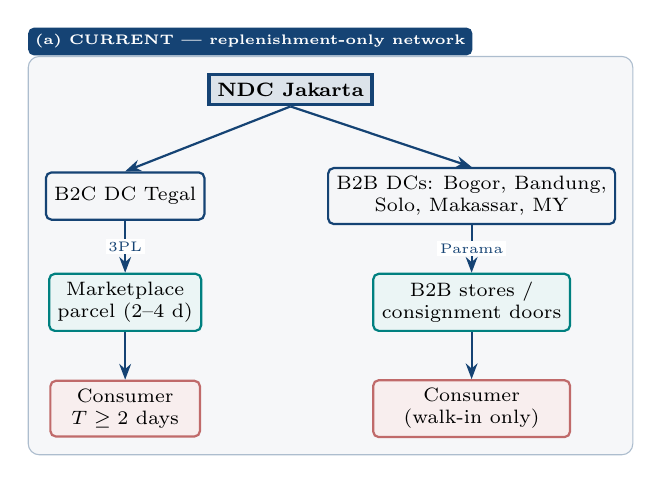
\begin{tikzpicture}
% ---- (a) current state ----
\node[node0, minimum width=20mm] (ndc) at (2.2,0) {NDC Jakarta};
\node[box, minimum width=19mm] (b2c) at (0.1,-1.35) {B2C DC Tegal};
\node[box, minimum width=25mm] (b2b) at (4.5,-1.35) {B2B DCs: Bogor, Bandung,\\Solo, Makassar, MY};
\node[ext, minimum width=19mm] (mp) at (0.1,-2.7) {Marketplace\\parcel (2--4 d)};
\node[ext, minimum width=25mm] (store) at (4.5,-2.7) {B2B stores /\\consignment doors};
\node[box, minimum width=19mm, fill=pxred!8, draw=pxred!70] (cons1) at (0.1,-4.05) {Consumer\\$T \ge 2$ days};
\node[box, minimum width=25mm, fill=pxred!8, draw=pxred!70] (cons2) at (4.5,-4.05) {Consumer\\(walk-in only)};
\draw[flow] (ndc.south) -- (b2c.north);
\draw[flow] (ndc.south) -- (b2b.north);
\draw[flow] (b2c) -- node[lbl]{3PL} (mp);
\draw[flow] (b2b) -- node[lbl]{Parama} (store);
\draw[flow] (mp) -- (cons1);
\draw[flow] (store) -- (cons2);
\begin{scope}[on background layer]
\node[panel=pxblue, fit=(ndc)(b2c)(b2b)(mp)(store)(cons1)(cons2)] (pa) {};
\end{scope}
\node[tab=pxblue] at (pa.north west) {(a) CURRENT --- replenishment-only network};
\end{tikzpicture}

\vspace{2.5mm}

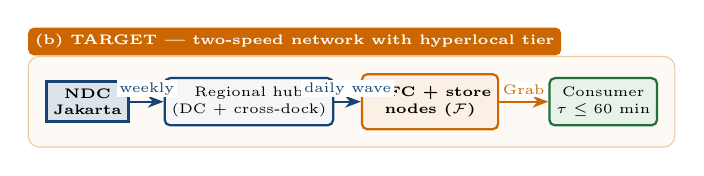
\begin{tikzpicture}
% ---- (b) target state ----
\node[node0, font=\tiny\bfseries, inner sep=2.5pt] (ndc2) at (0,0) {NDC\\Jakarta};
\node[box, font=\tiny, inner sep=2.5pt] (hub) at (2.05,0) {Regional hub\\(DC + cross-dock)};
\node[newsys, font=\tiny\bfseries, inner sep=2.5pt] (mfc) at (4.35,0) {MFC + store\\nodes ($\mathcal{F}$)};
\node[box, fill=pxgreen!10, draw=pxgreen, font=\tiny, inner sep=2.5pt] (c3) at (6.55,0) {Consumer\\$\tau \le 60$ min};
\draw[flow] (ndc2) -- node[lbl, above=0.4mm]{weekly} (hub);
\draw[flow] (hub) -- node[lbl, above=0.4mm]{daily wave} (mfc);
\draw[flow3] (mfc) -- node[lbl, above=0.4mm]{Grab} (c3);
\begin{scope}[on background layer]
\node[panel=pxorange, fit=(ndc2)(hub)(mfc)(c3)] (pb) {};
\end{scope}
\node[tab=pxorange] at (pb.north west) {(b) TARGET --- two-speed network with hyperlocal tier};
\end{tikzpicture}
\caption{From a replenishment network to a two-speed network. The existing backbone (a) is preserved; a hyperlocal fulfillment tier (b) is superimposed for the instant promise.}
\label{fig:current}
\end{figure}

\begin{figure*}[!t]
\centering
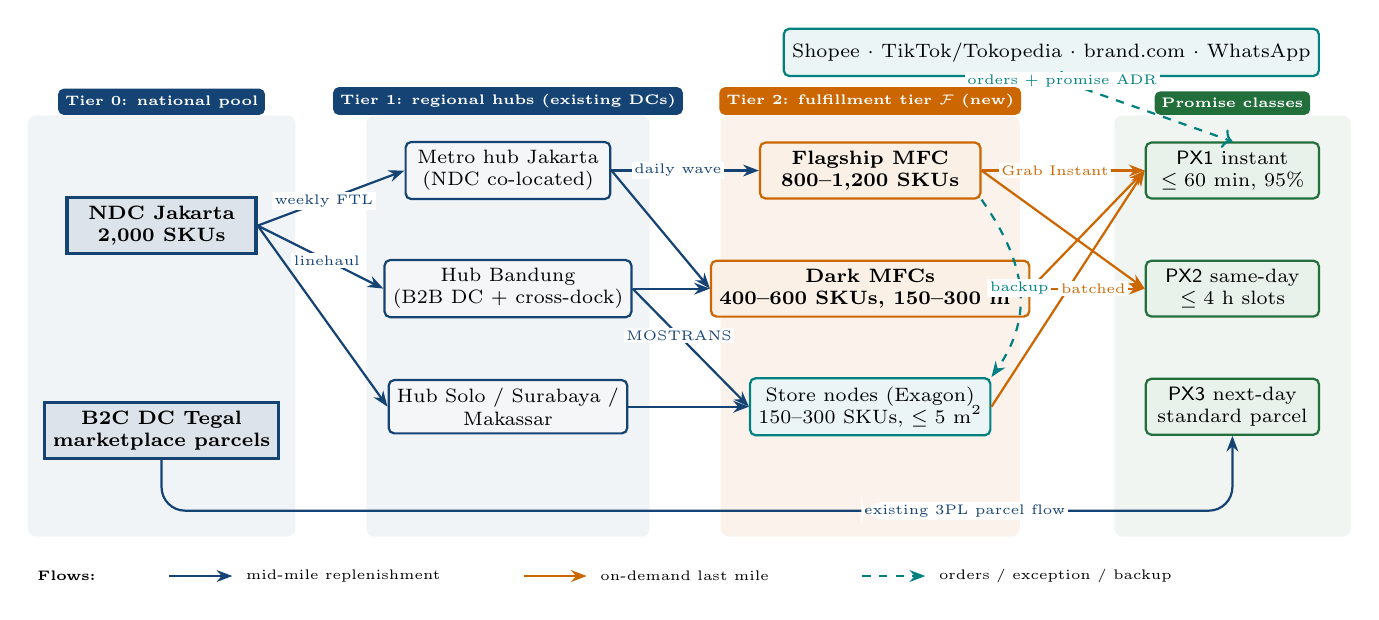
\begin{tikzpicture}
% Tier 0
\node[node0, minimum width=24mm] (ndc) at (0,0) {NDC Jakarta\\\scriptsize 2{,}000 SKUs};
\node[node0, minimum width=24mm] (tegal) at (0,-2.6) {B2C DC Tegal\\\scriptsize marketplace parcels};
% Tier 1
\node[box, minimum width=26mm] (hubjkt) at (4.4,0.7) {Metro hub Jakarta\\(NDC co-located)};
\node[box, minimum width=26mm] (hubbdg) at (4.4,-0.8) {Hub Bandung\\(B2B DC + cross-dock)};
\node[box, minimum width=26mm] (hubsolo) at (4.4,-2.3) {Hub Solo / Surabaya /\\Makassar};
% Tier 2
\node[newsys, minimum width=28mm] (flag) at (9.0,0.7) {Flagship MFC\\\scriptsize 800--1{,}200 SKUs};
\node[newsys, minimum width=28mm] (dark) at (9.0,-0.8) {Dark MFCs\\\scriptsize 400--600 SKUs, 150--300 m$^2$};
\node[ext, minimum width=28mm] (snode) at (9.0,-2.3) {Store nodes (Exagon)\\\scriptsize 150--300 SKUs, $\le 5$ m$^2$};
% Promise classes
\node[box, fill=pxgreen!10, draw=pxgreen, minimum width=22mm] (px1) at (13.6,0.7) {$\mathsf{PX1}$ instant\\$\le 60$ min, 95\%};
\node[box, fill=pxgreen!10, draw=pxgreen, minimum width=22mm] (px2) at (13.6,-0.8) {$\mathsf{PX2}$ same-day\\$\le 4$ h slots};
\node[box, fill=pxgreen!10, draw=pxgreen, minimum width=22mm] (px3) at (13.6,-2.3) {$\mathsf{PX3}$ next-day\\standard parcel};
% channels above
\node[ext, minimum width=40mm] (chan) at (11.3,2.2) {Shopee $\cdot$ TikTok/Tokopedia $\cdot$ brand.com $\cdot$ WhatsApp};
% mid-mile flows
\draw[flow] (ndc.east) -- node[lbl, pos=0.45]{weekly FTL} (hubjkt.west);
\draw[flow] (ndc.east) -- node[lbl, pos=0.55]{linehaul} (hubbdg.west);
\draw[flow] (ndc.east) -- (hubsolo.west);
\draw[flow] (hubjkt.east) -- node[lbl, pos=0.45]{daily wave} (flag.west);
\draw[flow] (hubjkt.east) -- (dark.west);
\draw[flow] (hubbdg.east) -- (dark.west);
\draw[flow] (hubbdg.east) -- node[lbl, pos=0.4]{MOSTRANS} (snode.west);
\draw[flow] (hubsolo.east) -- (snode.west);
% last mile
\draw[flow3] (flag.east) -- node[lbl, pos=0.45]{Grab Instant} (px1.west);
\draw[flow3] (dark.east) -- (px1.west);
\draw[flow3] (snode.east) -- (px1.west);
\draw[flow3] (dark.east) -- node[lbl, pos=0.55]{batched} (px2.west);
\draw[flow3] (flag.east) -- (px2.west);
% Tegal lane under everything
\draw[flow, rounded corners=3mm] (tegal.south) |- (6.8,-3.62) -| node[lbl, pos=0.25]{existing 3PL parcel flow} (px3.south);
% backup arc
\draw[flow2] (flag.south east) to[out=-55, in=55, looseness=1.1] node[lbl, pos=0.5]{backup} (snode.north east);
% channel orders
\draw[flow2, <->] (chan.south) -- node[lbl, pos=0.06]{orders + promise ADR} (px1.north);
% lanes
\begin{scope}[on background layer]
\fill[lane=pxblue!6]   (-1.7,-3.95) rectangle (1.7,1.4);
\fill[lane=pxblue!6]   (2.6,-3.95)  rectangle (6.2,1.4);
\fill[lane=pxorange!8] (7.1,-3.95)  rectangle (10.9,1.4);
\fill[lane=pxgreen!7]  (12.1,-3.95) rectangle (15.1,1.4);
\end{scope}
\node[lanetab=pxblue]   at (0,1.4)    {Tier 0: national pool};
\node[lanetab=pxblue]   at (4.4,1.4)  {Tier 1: regional hubs (existing DCs)};
\node[lanetab=pxorange] at (9.0,1.4)  {Tier 2: fulfillment tier $\mathcal{F}$ (new)};
\node[lanetab=pxgreen]  at (13.6,1.4) {Promise classes};
% legend
\node[font=\tiny, anchor=west] (lg0) at (-1.7,-4.45) {\textbf{Flows:}};
\draw[flow] (0.1,-4.45) -- (0.9,-4.45); \node[font=\tiny, anchor=west] at (0.95,-4.45) {mid-mile replenishment};
\draw[flow3] (4.6,-4.45) -- (5.4,-4.45); \node[font=\tiny, anchor=west] at (5.45,-4.45) {on-demand last mile};
\draw[flow2] (8.9,-4.45) -- (9.7,-4.45); \node[font=\tiny, anchor=west] at (9.75,-4.45) {orders / exception / backup};
\end{tikzpicture}
\caption{ParaExpress target network topology. Solid blue arcs: mid-mile replenishment; orange arcs: on-demand last mile; dashed teal: exception/backup flows. Tier~2 combines dedicated dark MFCs with activated Exagon consignment stores; the existing Tegal B2C flow continues to serve the standard promise unchanged.}
\label{fig:topology}
\end{figure*}

\subsection{Promise Tiers and Routing Waterfall}
Table~\ref{tab:sla} defines the promise portfolio. The routing waterfall implements graceful degradation: if no $\mathsf{PX1}$-feasible node passes the ATP and capacity filters of $(\mathsf{P3})$, the order is re-quoted as $\mathsf{PX2}$ (fulfilled by the flagship MFC in a batched Grab multi-stop run per Remark~\ref{rem:batching}) and otherwise as $\mathsf{PX3}$ from Tegal. The consumer always sees an honest, dynamically computed promise \emph{before} checkout---the single most important conversion lever observed across all benchmarks in Section~\ref{sec:benchmark}.

\begin{table}[!t]
\caption{ParaExpress Promise Portfolio}
\label{tab:sla}
\centering
\scriptsize
\begin{tabularx}{\columnwidth}{@{}l l l X@{}}
\toprule
\textbf{Class} & \textbf{Promise} $(\tau,\alpha)$ & \textbf{Fulfilled by} & \textbf{Last mile} \\
\midrule
$\mathsf{PX1}$ & $\le$60 min, 95\% & Store node / dark MFC & Grab Instant / GoSend on-demand \\
$\mathsf{PX2}$ & $\le$4 h slot, 95\% & Dark / flagship MFC & Batched multi-stop rider runs \\
$\mathsf{PX3}$ & Next day, 98\% & B2C DC Tegal & Existing 3PL parcel \\
$\mathsf{PXB}$ & B2B next-visit & Regional hubs & Parama / MOSTRANS \\
\bottomrule
\end{tabularx}
\end{table}

\section{MFC Operating Model}
\label{sec:fc}
The MFC is the unit of replication; its operating model is derived directly from Section~\ref{sec:theory}.

\subsection{Location Strategy: Strategic, Not Expensive}
Proposition~\ref{prop:floor} shows the binding quantity is the \emph{drive-time radius} $R = v(\tau - T_{\mathrm{route}} - t^{\alpha}_{\mathrm{node}})^+$, not street frontage. Because an MFC has no walk-in traffic, it can occupy Class-B/C space---inner second-row shophouses (\emph{ruko}), light-industrial mezzanines, or the back rooms of existing consignment partners---selected by three filters: (i)~centroid of a demand cell in the $(\mathsf{P1})$ solution; (ii)~motorcycle access to arterials in all catchment directions (isochrone, not Euclidean, coverage); (iii)~rent $\le$~30--40\% of equivalent retail frontage. This is the same cost logic that makes dark stores viable in Jakarta for quick-commerce operators, but with a beauty-specific advantage: no cold chain, low weight, high value density (a full motorcycle box of cosmetics can exceed the retail value of a full grocery van).

\subsection{Format Ladder and Assortment}
Table~\ref{tab:formats} specifies the three Tier-2 formats. Assortments are computed per node by Theorem~\ref{thm:assortment}: rank SKUs by catchment-level captured revenue rate $r_{fk}$ (from MagPie history projected to the catchment by ParaTwin's demand model), fill the slot budget, then apply brand-block completion so that advertised ``hero'' baskets (e.g., a Wardah skincare regimen bundle) are never split. A weekly re-optimization reallocates slow slots; beauty's low obsolescence makes mis-slotting cheap to reverse via the next replenishment wave.

\begin{table}[!t]
\caption{Tier-2 Fulfillment Node Formats}
\label{tab:formats}
\centering
\scriptsize
\begin{tabularx}{\columnwidth}{@{}l l l l@{}}
\toprule
& \textbf{Store node} & \textbf{Dark MFC} & \textbf{Flagship MFC} \\
\midrule
Space & $\le$5 m$^2$ in-store & 150--300 m$^2$ & 400--600 m$^2$ \\
SKUs (slots) & 150--300 & 400--600 & 800--1{,}200 \\
Fixed cost & $\approx$0 (rev.\ share) & low (Class-B/C rent) & moderate \\
Staffing & store staff & 2--6 pickers/shift & 4--10 pickers/shift \\
Throughput $\mu_f$ & 5--10 orders/h & 20--60 orders/h & 60--150 orders/h \\
Pick time target & $\le$7 min & $\le$5 min & $\le$5 min \\
Role & coverage endowment & $\mathsf{PX1}$ workhorse & long tail + $\mathsf{PX2}$ \\
Systems & Exagon + PX app & Heron~Lite & Heron~Lite \\
\bottomrule
\end{tabularx}
\end{table}

\subsection{In-Node Process and Layout}
Fig.~\ref{fig:mfclayout} shows the reference dark-MFC layout. The design target from Proposition~\ref{prop:floor} is $t^{\alpha}_{\mathrm{node}} \le 10$~min ($T_{\mathrm{queue}} \le 2$, $T_{\mathrm{pick}} \le 5$, $T_{\mathrm{handover}} \le 3$), achieved with: velocity-slotted shelving (top-50 SKUs within 3~m of the pack bench, mirroring the 2--3-minute pick discipline of Indian quick commerce); single-piece-flow pick carts with pick-to-light-lite (phone flash + shelf QR); pre-printed courier bags by promise class; and \emph{courier pre-matching}---the Grab booking is fired at pick start, not pack end, overlapping $T_{\mathrm{handover}}$ with $T_{\mathrm{pick}}$ (Section~\ref{sec:systems}). Staffing per shift follows the square-root rule \eqref{eq:staff}; ParaTwin continuously re-estimates $\nu$ and $\lambda_f$ and publishes next-week rosters.

\begin{figure}[!t]
\centering
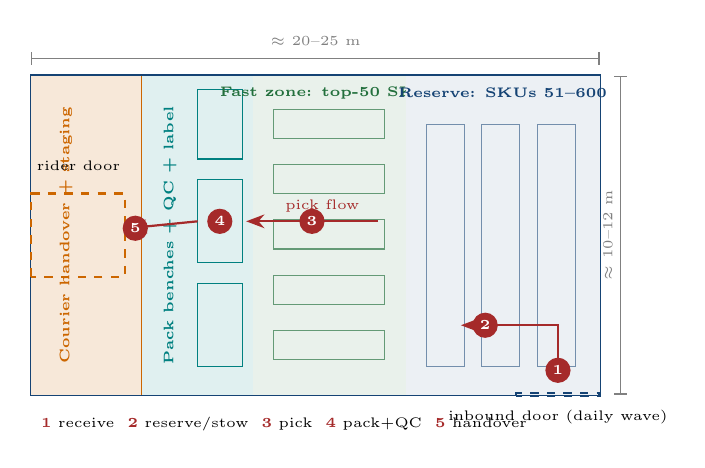
\begin{tikzpicture}[scale=0.88, every node/.style={font=\tiny}]
% outer wall
\draw[very thick, pxblue] (0,0) rectangle (8.2,4.6);
% dock / handover
\fill[pxorange!15] (0,0) rectangle (1.6,4.6);
\draw[pxorange, thick] (1.6,0) -- (1.6,4.6);
\node[rotate=90, font=\tiny\bfseries, pxorange] at (0.5,2.3) {Courier handover + staging};
\draw[pxorange, thick, dashed] (0,1.7) rectangle (1.35,2.9);
\node at (0.68,3.3) {rider door};
% pack zone
\fill[pxteal!12] (1.6,0) rectangle (3.2,4.6);
\node[rotate=90, font=\tiny\bfseries, pxteal] at (2.0,2.3) {Pack benches + QC + label};
\draw[pxteal] (2.4,0.4) rectangle (3.05,1.6);
\draw[pxteal] (2.4,1.9) rectangle (3.05,3.1);
\draw[pxteal] (2.4,3.4) rectangle (3.05,4.4);
% fast pick zone
\fill[pxgreen!10] (3.2,0) rectangle (5.4,4.6);
\node[font=\tiny\bfseries, pxgreen] at (4.3,4.35) {Fast zone: top-50 SKUs};
\foreach \y in {0.5,1.3,2.1,2.9,3.7} {\draw[pxgreen!70] (3.5,\y) rectangle (5.1,\y+0.42);}
% reserve zone
\fill[pxblue!8] (5.4,0) rectangle (8.2,4.6);
\node[font=\tiny\bfseries, pxblue] at (6.8,4.35) {Reserve: SKUs 51--600};
\foreach \x in {5.7,6.5,7.3} {\draw[pxblue!60] (\x,0.4) rectangle (\x+0.55,3.9);}
% receiving
\draw[pxblue, thick, dashed] (7.0,-0.02) rectangle (8.2,0.02);
\node at (7.6,-0.32) {inbound door (daily wave)};
% flow arrows with stage badges
\draw[-{Stealth}, thick, pxred] (7.6,0.35) -- (7.6,1.0) -- (6.2,1.0);
\draw[-{Stealth}, thick, pxred] (5.0,2.5) -- (3.1,2.5);
\draw[-{Stealth}, thick, pxred] (2.4,2.5) -- (1.4,2.4);
\node[pxred] at (4.2,2.72) {pick flow};
\node[badge] at (7.6,0.35) {1};
\node[badge] at (6.55,1.0) {2};
\node[badge] at (4.05,2.5) {3};
\node[badge] at (2.72,2.5) {4};
\node[badge] at (1.5,2.4) {5};
\node[font=\tiny, align=left, anchor=north west] at (0,-0.18)
  {\textcolor{pxred}{\textbf{1}} receive \ \textcolor{pxred}{\textbf{2}} reserve/stow \ \textcolor{pxred}{\textbf{3}} pick \ \textcolor{pxred}{\textbf{4}} pack+QC \ \textcolor{pxred}{\textbf{5}} handover};
% dimensions
\draw[dim] (0,4.85) -- node[above=0.3mm, font=\tiny, gray]{$\approx$ 20--25 m} (8.2,4.85);
\draw[dim] (8.5,0) -- node[right=0.3mm, font=\tiny, gray, rotate=90, anchor=south]{$\approx$ 10--12 m} (8.5,4.6);
\end{tikzpicture}
\caption{Reference dark-MFC layout (150--300 m$^2$). Material flows right-to-left through five stages: \textbf{1}~inbound wave receipt, \textbf{2}~reserve stow, \textbf{3}~pick (top-50 velocity SKUs adjacent to pack), \textbf{4}~pack + QC, \textbf{5}~courier handover---holding $T_{\mathrm{pick}} \le 5$ min.}
\label{fig:mfclayout}
\end{figure}

\subsection{Node Economics}
Table~\ref{tab:econ} gives the illustrative steady-state P\&L per dark MFC that ParaTwin must validate before each opening (values are design targets, not commitments; IDR figures indexed to 2026 Jakarta Class-B/C rents). The break-even logic follows the quick-commerce literature: contribution per order must cover rider fee net of consumer delivery fee plus pick cost, and daily volume must amortize the fixed base. Because beauty AOV (IDR~150--350k) is 2--4$\times$ grocery quick-commerce AOV while parcels are small, the model clears break-even at materially lower order density than grocery dark stores---the central reason a \emph{category-specialist} network can win where generalists struggle.

\begin{table}[!t]
\caption{Illustrative Dark-MFC Monthly Economics (Design Targets)}
\label{tab:econ}
\centering
\scriptsize
\begin{tabularx}{\columnwidth}{@{}X r@{}}
\toprule
\textbf{Item} & \textbf{Value} \\
\midrule
Orders/day (steady state) & 250 \\
Average order value (AOV) & IDR 220{,}000 \\
Gross margin before fulfillment & 40--55\% (owned brands) \\
Rider fee net of delivery fee charged & IDR 8{,}000--14{,}000 /order \\
Pick--pack labor (sq-root staffed) & IDR 4{,}000--6{,}000 /order \\
Rent + utilities (Class B/C, 200 m$^2$) & IDR 35--60M /month \\
Shrinkage + cycle-count allowance & $\le$0.3\% of sales \\
Contribution after fulfillment & IDR 55{,}000--90{,}000 /order \\
Fixed-cost break-even & $\approx$40--80 orders/day \\
\bottomrule
\end{tabularx}
\end{table}

\section{Business Model and Strategic Partnerships}
\label{sec:business}
\subsection{The B2C Business Model}
ParaExpress is a \emph{fulfillment capability}, not a new storefront. ParagonCorp does not attempt to out-app Shopee; it makes every existing channel faster:

\begin{itemize}[leftmargin=*]
  \item \textbf{Marketplace instant (primary).} On Shopee and TikTok Shop/Tokopedia, official ParagonCorp brand stores enroll in each platform's instant/same-day program. The marketplace remains the demand front end and payment rail; the order is fulfilled by the nearest ParaExpress node, with the platform's instant courier (SPX Instant) or a ParaExpress-booked Grab/GoSend rider performing the last mile according to the program's integration mode. ParagonCorp gains the buy-box advantage of the fastest promise \emph{within} the platform instead of competing against it.
  \item \textbf{Direct channels.} Brand.com sites and WhatsApp commerce quote the $\mathsf{PX1}$/$\mathsf{PX2}$ promise natively via the Promise API, capturing full margin and first-party data.
  \item \textbf{O2O for consignment partners.} A store node also serves \emph{its own} walk-in customers' delivery requests (``kirim sekarang''), giving partner stores an instant-commerce capability they could not build alone---the incentive that makes the consignment-FC program attractive to partners.
  \item \textbf{B2B synergy.} The same nodes take same-day emergency replenishment orders from nearby B2B doors (a salon that runs out of a Kahf line on a weekend), monetizing idle inter-peak capacity.
\end{itemize}

Revenue mechanics per order: consumer pays a delivery fee (subsidizable as a promotion lever); ParagonCorp captures manufacturer-plus-retail margin on direct channels or manufacturer margin plus avoided marketplace fulfillment fees on marketplaces; store nodes earn a per-order fulfillment fee plus their consignment margin, settled through Exagon. Because the goods are ParagonCorp's own brands, every basket carries structurally higher contribution than a reseller dark store shipping third-party goods---the decisive difference from Astro's economics.

\subsection{Strategic Partnership Topology}
Fig.~\ref{fig:partners} and Table~\ref{tab:partners} define the partnership model under principle P-5: \emph{partner the commodity, own the algorithm}.

\begin{table}[!t]
\caption{Partnership Model and Contract Structure}
\label{tab:partners}
\centering
\scriptsize
\begin{tabularx}{\columnwidth}{@{}l X X@{}}
\toprule
\textbf{Partner} & \textbf{Role} & \textbf{Contract / integration} \\
\midrule
Shopee, TikTok Shop/Tokopedia & Demand front end; instant program enrollment & Seller-fulfilled instant SLA programs; order webhooks to MagPie; promise ADR feed \\
MOSTRANS & Mid-mile: hub$\to$node daily waves; inter-hub transfers & Per-route tariff with SLA penalties; e-POD + GPS telemetry into ShipGo; CDOB-grade handling \\
Grab (GrabExpress) & Primary on-demand last mile & INSTANT/SAME\_DAY API; volume-tiered per-km rates; courier pre-matching; webhook tracking \\
GoSend (GoTo) & Secondary last mile; Tokopedia-native flow & Instant/Same-Day API; failover carrier in ShipGo rate shop \\
Consignment stores (Exagon) & Store nodes: forward stock + pick labor & Addendum to consignment agreement: reserved stock, pick SLA, per-order fee, cycle-count duty \\
Parama & Metro linehaul, returns, cash logistics & Captive capacity, scheduled milk runs \\
\bottomrule
\end{tabularx}
\end{table}

Dual-carrier last mile (Grab primary, GoSend failover) is deliberate: Theorem~\ref{thm:routing}'s cost coefficients $c_{of}$ are re-quoted per order across carriers by ShipGo's rate shop, keeping per-km pricing competitive and providing surge resilience. An own-fleet option (motorcycle couriers on ParaExpress payroll) is evaluated in ParaTwin as a scenario, but is \emph{not} recommended for launch: at launch volumes the utilization needed to beat Grab's marginal per-km cost is not attainable outside the top-3 Jakarta clusters, and fleet management is not ParagonCorp's comparative advantage. The decision rule is stated explicitly: own-fleet becomes attractive in a cluster only when sustained demand exceeds ${\sim}$35--45 orders/day per dedicated rider-equivalent at $\ge$70\% working-hour utilization---a threshold ParaTwin monitors per cluster.

\begin{figure}[!t]
\centering
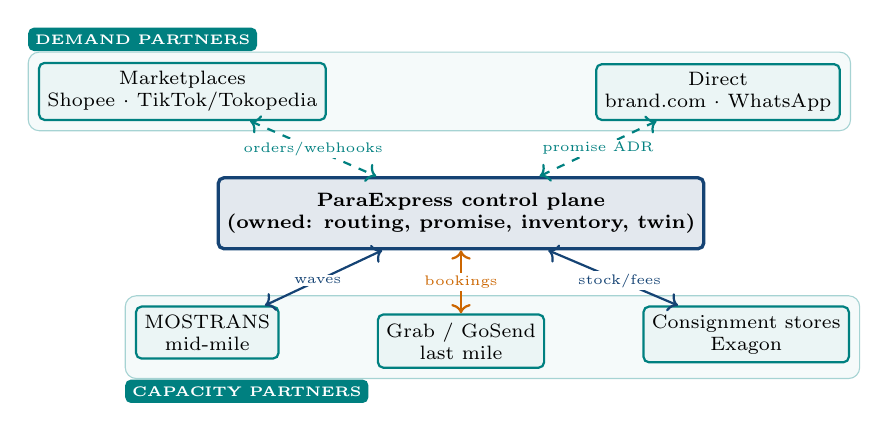
\begin{tikzpicture}[node distance=4mm and 6mm]
\node[sys, minimum width=34mm, minimum height=9mm, fill=pxblue!12, very thick] (px) {ParaExpress control plane\\\scriptsize (owned: routing, promise, inventory, twin)};
\node[ext, above left=7mm and -14mm of px, minimum width=19mm] (mkt) {Marketplaces\\\scriptsize Shopee $\cdot$ TikTok/Tokopedia};
\node[ext, above right=7mm and -14mm of px, minimum width=19mm] (direct) {Direct\\\scriptsize brand.com $\cdot$ WhatsApp};
\node[ext, below left=7mm and -8mm of px, minimum width=16mm] (mos) {MOSTRANS\\\scriptsize mid-mile};
\node[ext, below=8mm of px, minimum width=16mm] (grab) {Grab / GoSend\\\scriptsize last mile};
\node[ext, below right=7mm and -8mm of px, minimum width=16mm] (stores) {Consignment stores\\\scriptsize Exagon};
\draw[flow2, <->] (mkt) -- node[lbl]{orders/webhooks} (px);
\draw[flow2, <->] (direct) -- node[lbl]{promise ADR} (px);
\draw[flow, <->] (px) -- node[lbl, pos=0.55]{waves} (mos);
\draw[flow3, <->] (px) -- node[lbl]{bookings} (grab);
\draw[flow, <->] (px) -- node[lbl, pos=0.55]{stock/fees} (stores);
\begin{scope}[on background layer]
\node[panel=pxteal, fit=(mkt)(direct), inner sep=3.5pt] (bandD) {};
\node[panel=pxteal, fit=(mos)(grab)(stores), inner sep=3.5pt] (bandC) {};
\end{scope}
\node[tab=pxteal] at (bandD.north west) {DEMAND PARTNERS};
\node[tab=pxteal, anchor=north west] at (bandC.south west) {CAPACITY PARTNERS};
\end{tikzpicture}
\caption{Partnership topology. ParagonCorp owns the control plane (the algorithms and data); demand, mid-mile, and last-mile capacity are partnered.}
\label{fig:partners}
\end{figure}

\section{Solution Specification: Systems and Capabilities}
\label{sec:systems}
ParaExpress is realized by extending the four existing systems and adding three new platform services. Fig.~\ref{fig:sysarch} shows the target architecture; Fig.~\ref{fig:orderflow} the order lifecycle. The mapping is deliberate: each mathematical object of Section~\ref{sec:model} has exactly one system of record---$(\mathsf{P1})$/$(\mathsf{P2})$ live in ParaTwin, $(\mathsf{P3})$ in the Order Routing Engine, ATP (Proposition~\ref{prop:atp}) in the Virtual Inventory Service, \eqref{eq:basestock} in replenishment planning, and \eqref{eq:staff} in Heron~Lite labor planning.

\begin{figure*}[!t]
\centering
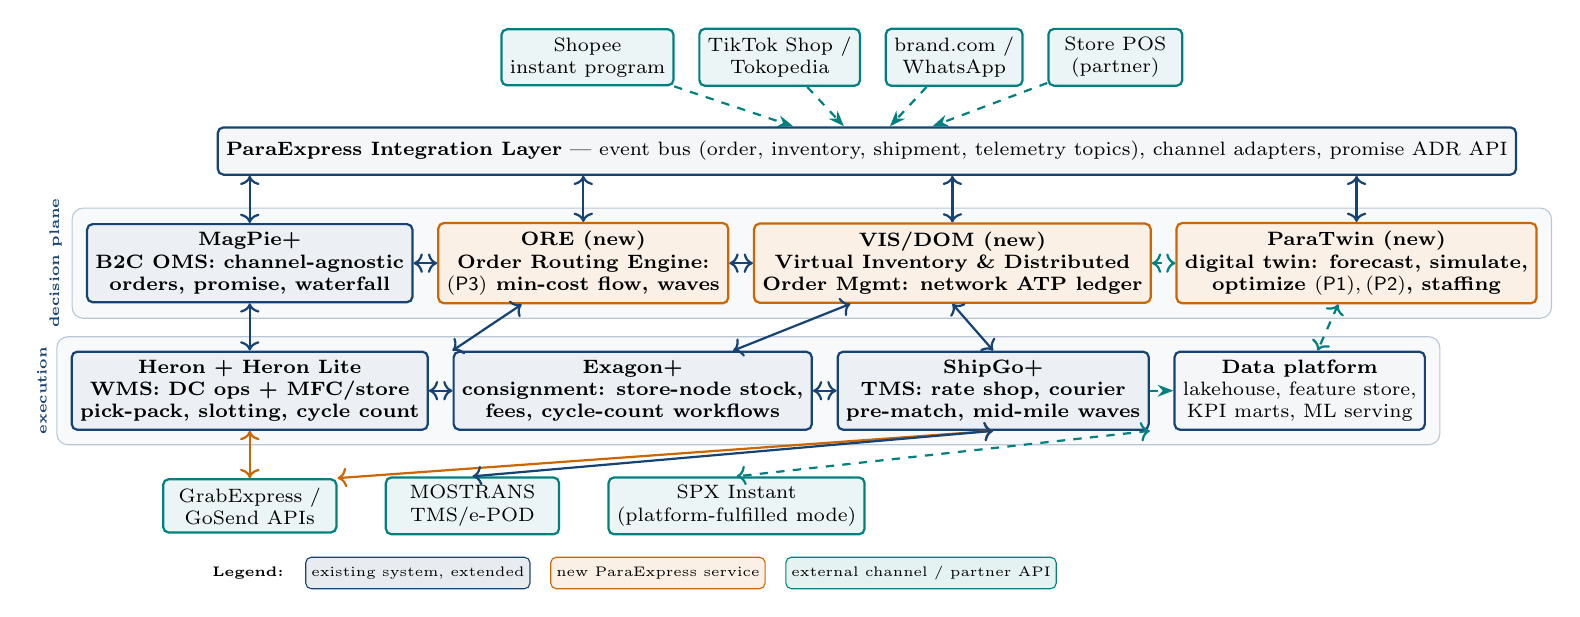
\begin{tikzpicture}[node distance=3.5mm and 5mm]
% channels layer
\node[ext, minimum width=19mm] (shopee) {Shopee\\\scriptsize instant program};
\node[ext, right=3mm of shopee, minimum width=19mm] (tiktok) {TikTok Shop /\\Tokopedia};
\node[ext, right=3mm of tiktok, minimum width=17mm] (brand) {brand.com /\\WhatsApp};
\node[ext, right=3mm of brand, minimum width=17mm] (pos) {Store POS\\\scriptsize (partner)};
% integration
\node[box, below=5mm of $(tiktok.south)!0.5!(brand.south)$, minimum width=86mm] (bus) {\textbf{ParaExpress Integration Layer} --- event bus (order, inventory, shipment, telemetry topics), channel adapters, promise ADR API};
% core row
\node[sys, below left=6mm and -25mm of bus, minimum width=24mm] (magpie) {\textbf{MagPie+}\\\scriptsize B2C OMS: channel-agnostic\\orders, promise, waterfall};
\node[newsys, right=3mm of magpie, minimum width=24mm] (ore) {\textbf{ORE} (new)\\\scriptsize Order Routing Engine:\\$(\mathsf{P3})$ min-cost flow, waves};
\node[newsys, right=3mm of ore, minimum width=24mm] (vis) {\textbf{VIS/DOM} (new)\\\scriptsize Virtual Inventory \& Distributed\\Order Mgmt: network ATP ledger};
\node[newsys, right=3mm of vis, minimum width=24mm] (twin) {\textbf{ParaTwin} (new)\\\scriptsize digital twin: forecast, simulate,\\optimize $(\mathsf{P1}),(\mathsf{P2})$, staffing};
% execution row
\node[sys, below=6mm of magpie, minimum width=24mm] (heron) {\textbf{Heron + Heron Lite}\\\scriptsize WMS: DC ops + MFC/store\\pick-pack, slotting, cycle count};
\node[sys, right=3mm of heron, minimum width=24mm] (exagon) {\textbf{Exagon+}\\\scriptsize consignment: store-node stock,\\fees, cycle-count workflows};
\node[sys, right=3mm of exagon, minimum width=24mm] (shipgo) {\textbf{ShipGo+}\\\scriptsize TMS: rate shop, courier\\pre-match, mid-mile waves};
\node[box, right=3mm of shipgo, minimum width=24mm] (data) {\textbf{Data platform}\\\scriptsize lakehouse, feature store,\\KPI marts, ML serving};
% partners bottom
\node[ext, below=6mm of heron, minimum width=22mm] (grabapi) {GrabExpress /\\GoSend APIs};
\node[ext, right=6mm of grabapi, minimum width=22mm] (mosapi) {MOSTRANS\\TMS/e-POD};
\node[ext, right=6mm of mosapi, minimum width=22mm] (spxapi) {SPX Instant\\\scriptsize (platform-fulfilled mode)};
% edges channels->bus
\draw[flow2] (shopee) -- (bus);
\draw[flow2] (tiktok) -- (bus);
\draw[flow2] (brand) -- (bus);
\draw[flow2] (pos) -- (bus);
% bus->core
\draw[flow, <->] (bus.south -| magpie) -- (magpie);
\draw[flow, <->] (bus.south -| ore) -- (ore);
\draw[flow, <->] (bus.south -| vis) -- (vis);
\draw[flow, <->] (bus.south -| twin) -- (twin);
% core interconnect
\draw[flow, <->] (magpie) -- (ore);
\draw[flow, <->] (ore) -- (vis);
\draw[flow2, <->] (vis) -- (twin);
% core->execution
\draw[flow, <->] (magpie) -- (heron);
\draw[flow, <->] (vis) -- (exagon);
\draw[flow, <->] (ore) -- (exagon.north west);
\draw[flow, <->] (vis.south) -- (shipgo.north);
\draw[flow2, <->] (twin) -- (data);
\draw[flow, <->] (heron) -- (exagon);
\draw[flow, <->] (exagon) -- (shipgo);
\draw[flow2] (shipgo) -- (data);
% execution->partners
\draw[flow3, <->] (heron.south) -- (grabapi.north);
\draw[flow3, <->] (shipgo.south) -- (grabapi.north east);
\draw[flow, <->] (shipgo.south) -- (mosapi.north);
\draw[flow2, <->] (shipgo.south east) -- (spxapi.north);
\begin{scope}[on background layer]
\node[grp, fit=(magpie)(ore)(vis)(twin), label={[font=\tiny\bfseries, pxblue]left:{\rotatebox{90}{decision plane}}}] {};
\node[grp, fit=(heron)(exagon)(shipgo)(data), label={[font=\tiny\bfseries, pxblue]left:{\rotatebox{90}{execution}}}] {};
\end{scope}
% legend
\node[font=\tiny\bfseries, below=5mm of grabapi, xshift=-6mm, anchor=west] (lg) {Legend:};
\node[chip=pxblue, right=1.5mm of lg] (c1) {existing system, extended};
\node[chip=pxorange, right=2.5mm of c1] (c2) {new ParaExpress service};
\node[chip=pxteal, right=2.5mm of c2] (c3) {external channel / partner API};
\end{tikzpicture}
\caption{ParaExpress target system architecture. Blue: existing systems extended (MagPie, Heron, Exagon, ShipGo); orange: new services (ORE, VIS/DOM, ParaTwin); teal: external channels and partner APIs, integrated through a shared event bus.}
\label{fig:sysarch}
\end{figure*}

\begin{figure}[!t]
\centering
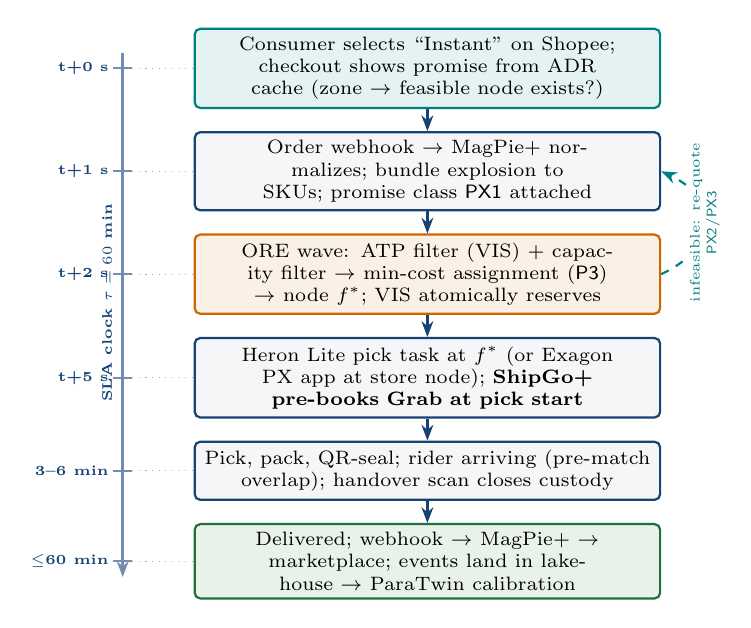
\begin{tikzpicture}[node distance=2.8mm and 4mm, every node/.style={font=\tiny}]
\node[box, text width=57mm, fill=pxteal!10, draw=pxteal] (s1) {Consumer selects ``Instant'' on Shopee; checkout shows promise from ADR cache (zone $\to$ feasible node exists?)};
\node[box, text width=57mm, below=of s1] (s2) {Order webhook $\to$ MagPie+ normalizes; bundle explosion to SKUs; promise class $\mathsf{PX1}$ attached};
\node[box, text width=57mm, below=of s2, fill=pxorange!10, draw=pxorange] (s3) {ORE wave: ATP filter (VIS) + capacity filter $\to$ min-cost assignment $(\mathsf{P3})$ $\to$ node $f^\ast$; VIS atomically reserves};
\node[box, text width=57mm, below=of s3] (s4) {Heron Lite pick task at $f^\ast$ (or Exagon PX app at store node); \textbf{ShipGo+ pre-books Grab at pick start}};
\node[box, text width=57mm, below=of s4] (s5) {Pick, pack, QR-seal; rider arriving (pre-match overlap); handover scan closes custody};
\node[box, text width=57mm, below=of s5, fill=pxgreen!10, draw=pxgreen] (s6) {Delivered; webhook $\to$ MagPie+ $\to$ marketplace; events land in lakehouse $\to$ ParaTwin calibration};
\foreach \a/\b in {s1/s2, s2/s3, s3/s4, s4/s5, s5/s6} {\draw[flow] (\a) -- (\b);}
% SLA clock axis
\coordinate (axtop) at ($(s1.west)+(-9mm,2mm)$);
\coordinate (axbot) at ($(s6.west)+(-9mm,-2mm)$);
\draw[-{Stealth[length=2mm]}, very thick, pxblue!60] (axtop) -- node[rotate=90, above=1.5mm, font=\tiny\bfseries, pxblue, pos=0.5]{SLA clock $\tau = 60$ min} (axbot);
\foreach \s/\t in {s1/{t+0 s}, s2/{t+1 s}, s3/{t+2 s}, s4/{t+5 s}, s5/{3--6 min}, s6/{$\le$60 min}} {
  \draw[pxblue!60, thick] ($(\s.west)+(-10.2mm,0)$) -- ($(\s.west)+(-7.8mm,0)$);
  \node[font=\tiny\bfseries, pxblue, anchor=east, inner sep=1pt] at ($(\s.west)+(-10.4mm,0)$) {\t};
  \draw[gray!60, dotted] ($(\s.west)+(-7.8mm,0)$) -- (\s.west);
}
% infeasibility feedback
\draw[flow2, dashed] (s3.east) to[out=25, in=-25, looseness=1.6] node[lbl, pos=0.5, rotate=90, align=center]{infeasible: re-quote\\$\mathsf{PX2}/\mathsf{PX3}$} (s2.east);
\end{tikzpicture}
\caption{$\mathsf{PX1}$ order lifecycle. Courier pre-matching at pick start overlaps $T_{\mathrm{handover}}$ with $T_{\mathrm{pick}}$, directly widening the feasible radius $R$ of Proposition~\ref{prop:floor}.}
\label{fig:orderflow}
\end{figure}

\subsection{MagPie+ (B2C Order Management System)}
MagPie remains the order system of record and gains the promise and orchestration features listed in Table~\ref{tab:magpie}.

\begin{table}[!t]
\caption{MagPie+ New Capabilities}
\label{tab:magpie}
\centering
\scriptsize
\begin{tabularx}{\columnwidth}{@{}l X@{}}
\toprule
\textbf{Feature} & \textbf{Specification} \\
\midrule
Promise API (ADR) & Available-to-deliver by zone $\times$ promise class, $\le$50 ms p99, pushed to channel adapters; computed from VIS ATP + ORE feasibility + Grab ETA feeds \\
Promise waterfall & $\mathsf{PX1} \to \mathsf{PX2} \to \mathsf{PX3}$ degradation with re-quote, per Section~\ref{sec:network}; never promise-then-cancel \\
Bundle explosion & Bundles/gift sets resolved to component SKUs with co-location constraint (single-node fulfillment preferred, split shipment as exception) \\
Channel adapters & Shopee/TikTok-Tokopedia instant-program webhooks, brand.com, WhatsApp commerce; idempotent order ingestion, $\ge$99.95\% availability \\
Order state machine & Adds \textsc{routed}, \textsc{picking}, \textsc{courier\_matched}, \textsc{handover}, \textsc{delivered\_px} states with SLA clocks per state \\
NDR/returns & Failed-delivery re-attempt policy, node return-to-stock with QC gate in Heron Lite \\
SLA cockpit & Real-time $\alpha$-attainment per promise class/zone/node; breach root-cause tags (queue, pick, courier, traffic) feeding ParaTwin \\
\bottomrule
\end{tabularx}
\end{table}

\subsection{Heron Lite (MFC Warehouse Management)}
Full Heron is engineered for the Tegal parcel DC; MFCs need a stripped, tablet-first profile---\emph{Heron Lite}---sharing Heron's item master and stock ledger: wave-less single-order picking with dynamic pick-path (velocity slotting from Theorem~\ref{thm:assortment} outputs); QR shelf labels and scan-verified picks ($\ge$99.9\% pick accuracy target); pack-bench QC with photo evidence for marketplace dispute defense; blind cycle counting scheduled by ABC class (A daily, B weekly, C monthly); labor planning via \eqref{eq:staff} with shift templates; and offline-tolerant operation (store-and-forward) for connectivity dips. Design throughput: one picker sustains 10--14 orders/hour at the reference layout of Fig.~\ref{fig:mfclayout}.

\subsection{Exagon+ (Consignment System) --- the Store-Node Enabler}
Exagon already tracks consignment stock and settlement; activating stores as fulfillment nodes adds: (i)~\emph{reserved virtual location} per store---ParaExpress forward stock is a distinct ledger location, not commingled with floor stock, physically a locked shelf unit; (ii)~a \emph{PX store app} (Android) for accept/pick/pack/handover with per-step timers and photo QC; (iii)~\emph{POS sale posting} within latency $\ell \le 5$~min (API or app quick-entry) to honor Proposition~\ref{prop:atp}, with protection buffers $s_{fk}$ auto-tuned from each store's posting-latency history; (iv)~\emph{accuracy scoring}---stores are scored on cycle-count variance and pick SLA; scores gate their eligibility set in ORE (a low-accuracy store is quoted fewer orders, an incentive-compatible mechanism); (v)~\emph{settlement}---per-order pick fees and consignment margin in the existing statement cycle.

\subsection{ShipGo+ (Transportation Management System)}
ShipGo extends from mid-mile TMS to a dual-clock transport brain: (i)~\emph{on-demand module}---Grab/GoSend rate shop and booking with courier \emph{pre-matching} fired at pick start, ETA ingestion, webhook tracking, auto-failover between carriers, surge-aware carrier choice (the $c_{of}$ coefficients of $(\mathsf{P3})$ refresh per quote); (ii)~\emph{batched module}---$\mathsf{PX2}$ multi-stop rider runs built by a capacitated VRP heuristic (savings + 2-opt, $\le$8 stops) within promise windows \cite{tothvigo,klapp}; (iii)~\emph{mid-mile module}---daily replenishment waves hub$\to$nodes tendered to MOSTRANS with e-POD, temperature/handling flags, and SLA penalty tracking; (iv)~\emph{control tower}---courier exception detection (no-show, wrong-direction GPS) with automatic re-booking inside the SLA clock.

\subsection{VIS/DOM: Virtual Inventory \& Distributed Order Management (New)}
The VIS is the single linearizable ledger of Proposition~\ref{prop:atp}: network-wide ATP per (node, SKU, promise class) with atomic reserve/release, protection buffers, and event-sourced audit; sub-10~ms reserve latency; back-pressure semantics so a channel can never oversell a node. The DOM half owns cross-node policies: split-shipment rules, node-down rebalancing, safety-stock substitution (offer the 30~ml when the 50~ml is out, per brand rules), and marketplace stock-feed publication (per-node buffered availability instead of national availability---the change that makes marketplace instant programs \emph{honest}).

\subsection{ORE: Order Routing Engine (New)}
The ORE implements Theorem~\ref{thm:routing}: micro-batched min-cost-flow assignment over feasible (order, node) pairs with cost $c_{of} = $ courier quote $+$ congestion shadow price (queue-length-dependent) $+$ inventory-displacement penalty (from VIS safety positions) $-$ node-accuracy bonus. Deterministic solver, $\le$100~ms per wave, full decision logging (every routing decision is replayable in ParaTwin---the operational network and its twin share one decision codebase, eliminating model drift).

\subsection{Module Decomposition of the New Services}
Table~\ref{tab:modules} decomposes the three new services into modules with single responsibilities; each module traces to the mathematical object it implements.

\begin{table}[!t]
\caption{Module Decomposition of ORE, VIS/DOM, and ParaTwin}
\label{tab:modules}
\centering
\scriptsize
\begin{tabularx}{\columnwidth}{@{}l X X@{}}
\toprule
\textbf{Module} & \textbf{Responsibility} & \textbf{Core technique} \\
\midrule
\multicolumn{3}{@{}l}{\textbf{ORE --- Order Routing Engine}} \\
Feasibility filter & Build $\mathcal{F}(o)$: promise coverage, ATP probe, residual capacity & Geohash zone index; VIS bulk probe \\
Cost model & Compose $c_{of}$: courier quote, congestion, displacement, accuracy & Queue-length shadow prices \\
Solver core & Exact assignment per wave & SSP min-cost flow (Thm.~\ref{thm:routing}), warm start \\
Wave scheduler & Adaptive micro-batching $\Delta \in [5,30]$ s & Remark~\ref{rem:batching}; load-triggered \\
Decision log & Append-only, replayable decisions & Event sourcing; twin replay \\
\midrule
\multicolumn{3}{@{}l}{\textbf{VIS/DOM --- Virtual Inventory \& Distributed Order Mgmt}} \\
ATP ledger & Linearizable reserve/release per (node, SKU) & Atomic compare-and-decrement (Prop.~\ref{prop:atp}) \\
Buffer engine & Tune $s_{fk}$ from POS posting-latency history & Poisson tail targets \\
Reservation mgr & Reservation lifecycle with TTL and audit & Event-sourced state machine \\
Stock publisher & Per-node buffered ATP feeds to channels & Debounced push, $\le$30 s staleness \\
Rebalancer / DOM & Node-down reallocation, splits, substitution & Re-run $(\mathsf{P3})$ on affected orders \\
\midrule
\multicolumn{3}{@{}l}{\textbf{ParaTwin --- Digital Twin}} \\
Ingestion & Enforce Table~\ref{tab:contracts} contracts, freshness gates & Schema registry; $>$48 h staleness refusal \\
Calibration & Fit $\Theta$: demand, pick, ETA, latency & MLE / quantile regression \\
DES kernel & Simulate $\mathcal{T}$ at SKU grain & Event heap; CRN; $\ge$30 replications \\
Optimizer bank & Candidates for $(\mathsf{P1})$, $(\mathsf{P2})$, \eqref{eq:staff} & Greedy (Thm.~\ref{thm:submodular}), matroid/knapsack (Thm.~\ref{thm:assortment}) \\
Experiment mgr & Scenario DSL, portfolio E1--E6, ranking \& selection & Common random numbers \cite{law} \\
Certification & Trace-replay + holdout gates, monthly re-cert & $\le$10\% KPI deviation gate \\
\bottomrule
\end{tabularx}
\end{table}

\subsection{Interface Contracts: APIs and Events}
All inter-system communication is either a synchronous API on the critical path (Table~\ref{tab:apis}) or an asynchronous event on the bus (Table~\ref{tab:events}). Events are delivered at-least-once with idempotency keys and are partitioned by order/node identifier so per-entity ordering is preserved; every state-changing service writes through the transactional-outbox pattern so bus publication and database commit are atomic.

\begin{table}[!t]
\caption{Synchronous API Contracts (Critical Path)}
\label{tab:apis}
\centering
\scriptsize
\begin{tabularx}{\columnwidth}{@{}l l X l@{}}
\toprule
\textbf{API} & \textbf{Provider} & \textbf{Semantics} & \textbf{p99 / avail.} \\
\midrule
Promise quote & MagPie+ & zone + basket $\to$ promise class, ETA, fee & 50 ms / 99.95\% \\
ATP reserve & VIS & atomic multi-line reserve; all-or-nothing & 10 ms / 99.99\% \\
Route solve & ORE & wave batch $\to$ integral assignment & 100 ms / 99.9\% \\
Courier book & ShipGo+ & quote-and-book with failover chain & 2 s / 99.9\% \\
Node task push & Heron Lite / PX app & pick task w/ offline queue & 1 s / 99.5\% \\
Scenario run & ParaTwin & async job: design $\to$ KPI vector + CIs & batch \\
\bottomrule
\end{tabularx}
\end{table}

\begin{table}[!t]
\caption{Asynchronous Event Catalog (Bus Topics)}
\label{tab:events}
\centering
\scriptsize
\begin{tabularx}{\columnwidth}{@{}l >{\raggedright\arraybackslash}p{25mm} X@{}}
\toprule
\textbf{Topic} & \textbf{Producer $\to$ consumers} & \textbf{Key payload} \\
\midrule
\texttt{order.created} & Adapters $\to$ MagPie+, ORE & channel, basket, promise quote \\
\texttt{order.routed} & ORE $\to$ nodes, VIS, MagPie+ & node $f^\ast$, reservation ids, SLA clock \\
\texttt{atp.changed} & VIS $\to$ adapters, ParaTwin & node, SKU, buffered ATP delta \\
\texttt{pick.status} & Heron Lite / PX app $\to$ ShipGo+, MagPie+ & start/complete stamps, accuracy \\
\texttt{courier.status} & ShipGo+ $\to$ MagPie+, lakehouse & booked/arrived/delivered, GPS legs \\
\texttt{pos.sale} & Exagon+ $\to$ VIS & store, SKU, qty, posting latency $\ell$ \\
\texttt{wave.epod} & MOSTRANS via ShipGo+ $\to$ Heron Lite, VIS & receipt lines, OTIF, temperature \\
\texttt{sla.breach} & MagPie+ $\to$ ParaTwin, ops cockpit & stage, root-cause tag, magnitude \\
\bottomrule
\end{tabularx}
\end{table}

\subsection{Non-Functional Requirements and Deployment}
Table~\ref{tab:nfr} states the binding non-functional requirements. Deployment topology: stateless services on a container platform across two Jakarta availability zones (active--active), a Kafka-class event bus, and per-service databases; the VIS ledger runs single-writer-per-node-partition with synchronous replication (RPO~0), which preserves the linearizability premise of Proposition~\ref{prop:atp} without cross-partition coordination. Edge clients (Heron Lite tablets, Exagon PX app) are offline-tolerant with store-and-forward queues of $\ge$4~h; because each node's ledger partition has a single writer, offline replay is conflict-free. Security: mTLS + OAuth2 service auth, role-based access at node granularity, consumer PII minimized---delivery addresses are tokenized and materialized only in ShipGo+ at booking time, then purged after proof-of-delivery retention. Every state change is event-sourced, so the audit trail and the ParaTwin calibration feed are the same stream.

\begin{table}[!t]
\caption{Non-Functional Requirements per Service}
\label{tab:nfr}
\centering
\scriptsize
\begin{tabularx}{\columnwidth}{@{}l l l X@{}}
\toprule
\textbf{Service} & \textbf{Avail.} & \textbf{p99} & \textbf{Scale / recovery} \\
\midrule
MagPie+ & 99.95\% & 50 ms & 50 orders/s steady, 10$\times$ campaign burst; RTO 15 min \\
ORE & 99.9\% & 100 ms & $10^3$ orders/wave, $10^2$ nodes/metro; stateless replay \\
VIS/DOM & 99.99\% & 10 ms & 5k reservations/s; RPO 0 (sync repl.) \\
Heron Lite & 99.5\% & 1 s & offline $\ge$4 h store-and-forward \\
Exagon+ PX & 99.5\% & 1 s & POS posting $\ell \le 5$ min, monitored per store \\
ShipGo+ & 99.9\% & 2 s & carrier failover $\le$30 s; dual-carrier quotas \\
ParaTwin & batch & --- & $10^6$ events/s/replication; nightly master sync \\
\bottomrule
\end{tabularx}
\end{table}

\subsection{Capability Superiority Matrix}
Table~\ref{tab:superiority} states, feature by feature, how the specification is designed to exceed the benchmark operators' observable capabilities within the beauty category.

\begin{table}[!t]
\caption{ParaExpress vs.\ Benchmark Capabilities (Beauty Category)}
\label{tab:superiority}
\centering
\scriptsize
\begin{tabularx}{\columnwidth}{@{}X X X@{}}
\toprule
\textbf{Capability} & \textbf{Benchmark practice} & \textbf{ParaExpress specification} \\
\midrule
Promise computation & Static zone tables (most marketplaces) & Per-order ADR from live ATP + queue + courier ETA (Prop.~\ref{prop:floor}) \\
Node economics & Generalist dark store, low AOV & Own-brand margin, high value density; break-even at 40--80 orders/day (Tab.~\ref{tab:econ}) \\
Coverage capex & Leased dark stores only (Astro, SPX MFCs) & Zero-capex consignment activation first (Cor.~\ref{cor:stores}), MFCs fill gaps \\
Assortment & Store-level heuristics & Per-catchment optimal forward sets, weekly re-optimized (Thm.~\ref{thm:assortment}) \\
Routing & Nearest-node rules & Exact min-cost flow with congestion + displacement pricing (Thm.~\ref{thm:routing}) \\
Handover & Sequential pick-then-book & Courier pre-match at pick start (overlapped clocks) \\
Design governance & Ad hoc expansion & Twin-gated: no node opens without ParaTwin acceptance (Sec.~\ref{sec:twin}) \\
\bottomrule
\end{tabularx}
\end{table}

\section{ParaTwin: Digital Twin Design}
\label{sec:twin}
Theorem~\ref{thm:nphard} establishes that the design space cannot be exhaustively optimized; the benchmarks (JD's deployed forecast--optimize--simulate loop \cite{jdassort}, Amazon's regionalization program \cite{amazonregional}) establish that the winning practice is a calibrated simulation--optimization loop. ParaTwin is that loop for ParagonCorp, in the sense of the digital supply chain twin literature \cite{ivanov,lefan,snoeck}.

\subsection{Formal Model}
\begin{definition}[ParaTwin]
\label{def:twin}
ParaTwin is a discrete-event simulation \cite{law} defined by the tuple
$\mathcal{T} = (\mathcal{X}, \mathcal{E}, \Phi, \Theta, \mathcal{Y})$:
\begin{itemize}[leftmargin=*]
  \item \textbf{State} $\mathcal{X}$: inventory positions $I_{fk}(t)$ and reservations $Q_{fk}(t)$ for all $f \in \mathcal{F} \cup \mathcal{D} \cup \{0\}$, $k \in \mathcal{K}$; queue contents and picker occupancy per node; courier states (idle, to-pickup, to-drop); mid-mile shipments in transit; open orders with promise clocks.
  \item \textbf{Events} $\mathcal{E}$: order arrival (marked spatial Poisson, rates $\lambda_{zk}(t)$ with hour-of-day/day-of-week/campaign seasonality; basket sampler $\mathcal{B}_z$; live-commerce demand shocks modeled as Hawkes bursts), routing decision, pick start/end, courier match/arrive/depart/deliver, replenishment wave dispatch/receipt, POS sale at store nodes, cycle-count adjustment, node outage.
  \item \textbf{Dynamics} $\Phi$: the state-transition kernel; crucially, routing transitions call the \emph{same ORE codebase} as production, and ATP transitions the same VIS rules---the twin and the network share decision logic by construction.
  \item \textbf{Parameters} $\Theta$: pick-time distributions per format (lognormal, fitted from Heron Lite event logs), Grab/GoSend ETA and price distributions by zone-pair and hour (fitted from ShipGo quotes and outcomes), travel-time matrices from historical rider GPS, store posting-latency distributions (Exagon), demand model coefficients.
  \item \textbf{Outputs} $\mathcal{Y}$: the KPI vector of Table~\ref{tab:kpi} with confidence intervals from $\ge$30 independent replications (common random numbers across compared designs for variance reduction \cite{law}).
\end{itemize}
\end{definition}

\subsection{Scope: 16 Brands, ${\approx}2{,}000$ SKUs}
The twin is SKU-explicit, not aggregated: assortment decisions (Theorem~\ref{thm:assortment}), substitution, and bundle co-location effects are only visible at SKU granularity. Scale is tractable: $2{,}000$ SKUs $\times$ ${\sim}150$ nodes (national end-state) is a $3\times10^5$-cell inventory state---small for a modern DES engine ($10^6$+ events/s single-threaded). The item master (dimensions, slot class, brand block, halal lot/expiry attributes), bundle bill-of-materials, and brand campaign calendars are synchronized nightly from MagPie/Heron masters; ParaTwin refuses to run a scenario whose master-data snapshot is stale ($>$48~h), a governance rule that prevents the classic twin-drift failure.

\subsection{Calibration and Validation Data Contracts}
Each production system publishes a calibration feed (Table~\ref{tab:contracts}). Validation is two-stage: \emph{trace-driven replay}---feed one historical week of real orders through the twin and require per-KPI deviation $\le$10\% against actuals; then \emph{holdout forecasting}---simulate the next week ahead of time and score prediction intervals. A twin version is certified for decision use only after both gates pass; certification is re-run monthly.

\begin{table}[!t]
\caption{ParaTwin Calibration Data Contracts}
\label{tab:contracts}
\centering
\scriptsize
\begin{tabularx}{\columnwidth}{@{}l X l@{}}
\toprule
\textbf{Source} & \textbf{Feed} & \textbf{Cadence} \\
\midrule
MagPie+ & Orders, baskets, promises, SLA outcomes & streaming \\
Heron/Lite & Pick/pack event timestamps, accuracy, labor & streaming \\
Exagon+ & Store stock, POS postings, count variances & 5 min \\
ShipGo+ & Courier quotes, ETAs, actual legs, mid-mile e-POD & streaming \\
Grab/GoSend & Zone-pair ETA/price distributions & daily fit \\
MOSTRANS & Wave lead times, OTIF, temperature logs & per wave \\
Market data & Campaign calendar, live-commerce schedule & weekly \\
\bottomrule
\end{tabularx}
\end{table}

\subsection{Simulation--Optimization Loop}
Fig.~\ref{fig:twinarch} shows the loop. Candidate designs are generated by the greedy/matroid algorithms of Section~\ref{sec:theory} (fast, with guarantees), then evaluated in the twin under stochastic demand, courier variability, and disruption scenarios; a ranking-and-selection procedure picks the certified winner \cite{snoeck,law}. The loop runs at three cadences: \emph{strategic} (quarterly: node openings, $n^\star$ re-estimation per Fig.~\ref{fig:costcurve}), \emph{tactical} (weekly: assortments $S_f$, base stocks $b_{fk}$, rosters $c_f$), and \emph{operational} (daily shadow mode: the twin replays yesterday against alternative routing policies and flags regret $>$ threshold).

\begin{figure}[!t]
\centering
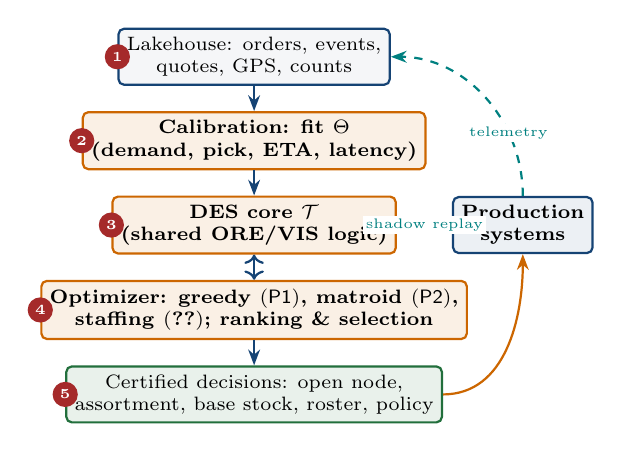
\begin{tikzpicture}[node distance=3.2mm and 5mm]
\node[box, minimum width=34mm] (data) {Lakehouse: orders, events,\\quotes, GPS, counts};
\node[newsys, below=of data, minimum width=34mm] (cal) {Calibration: fit $\Theta$\\(demand, pick, ETA, latency)};
\node[newsys, below=of cal, minimum width=34mm] (des) {DES core $\mathcal{T}$\\(shared ORE/VIS logic)};
\node[newsys, below=of des, minimum width=34mm] (opt) {Optimizer: greedy $(\mathsf{P1})$, matroid $(\mathsf{P2})$,\\staffing \eqref{eq:staff}; ranking \& selection};
\node[box, below=of opt, minimum width=34mm, fill=pxgreen!10, draw=pxgreen] (dec) {Certified decisions: open node,\\assortment, base stock, roster, policy};
\node[sys, right=7mm of des, minimum width=17mm] (prod) {Production\\systems};
\draw[flow] (data) -- (cal);
\draw[flow] (cal) -- (des);
\draw[flow, <->] (des) -- (opt);
\draw[flow] (opt) -- (dec);
\draw[flow3] (dec.east) to[out=0, in=-90] (prod.south);
\draw[flow2] (prod.north) to[out=90, in=0] node[lbl, pos=0.3]{telemetry} (data.east);
\draw[flow2, dashed] (prod) -- node[lbl]{shadow replay} (des);
\foreach \n/\i in {data/1, cal/2, des/3, opt/4, dec/5} {\node[badge] at (\n.west) {\i};}
\end{tikzpicture}
\caption{ParaTwin simulation--optimization loop. Production telemetry calibrates the twin; algorithmic design candidates are stress-tested in simulation; only certified decisions reach production; daily shadow replay detects drift.}
\label{fig:twinarch}
\end{figure}

\begin{figure}[!t]
\centering
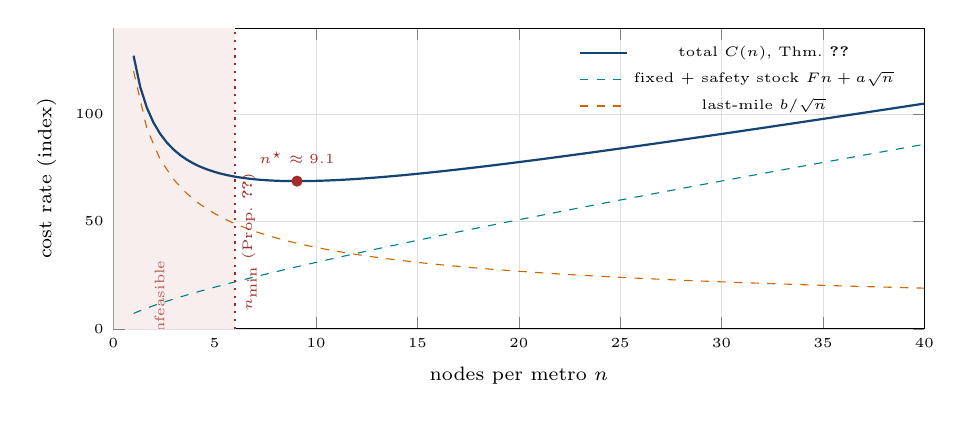
\begin{tikzpicture}
\begin{axis}[
  width=0.98\columnwidth, height=54mm,
  xlabel={nodes per metro $n$}, ylabel={cost rate (index)},
  xmin=0, xmax=40, ymin=0, ymax=140,
  label style={font=\scriptsize}, tick label style={font=\tiny},
  legend style={font=\tiny, at={(0.98,0.98)}, anchor=north east, draw=none, fill=none},
  grid=major, grid style={gray!25, very thin},
]
% F=1.2, a=6, b=120 (illustrative)
\fill[pxred!8] (axis cs:0,0) rectangle (axis cs:6,140);
\node[font=\tiny, pxred!80, rotate=90, anchor=south] at (axis cs:3,4) {SLA-infeasible};
\addplot[domain=1:40, samples=120, thick, pxblue] {1.2*x + 6*sqrt(x) + 120/sqrt(x)};
\addlegendentry{total $C(n)$, Thm.~\ref{thm:ncost}}
\addplot[domain=1:40, samples=60, dashed, pxteal] {6*sqrt(x)+1.2*x};
\addlegendentry{fixed + safety stock $Fn + a\sqrt{n}$}
\addplot[domain=1:40, samples=60, dashed, pxorange] {120/sqrt(x)};
\addlegendentry{last-mile $b/\sqrt{n}$}
\addplot[only marks, mark=*, mark size=1.8pt, pxred] coordinates {(9.06,68.8)};
\node[font=\tiny, pxred, anchor=south] at (axis cs:9.06,72) {$n^\star \approx 9.1$};
\addplot[dotted, thick, pxred] coordinates {(6,0) (6,140)};
\node[font=\tiny, pxred, anchor=west, rotate=90] at (axis cs:6.7,4) {$n_{\min}$ (Prop.~\ref{prop:floor})};
\end{axis}
\end{tikzpicture}
\caption{Illustrative ParaTwin design curve for one metro: unimodal total cost with unique $n^\star$ (Theorem~\ref{thm:ncost}) and the SLA feasibility floor $n_{\min}$; the network is sized at $\max(n_{\min}, n^\star)$. Validation: for $(F,a,b)=(1.2,6,120)$ the cubic $2Fx^3 + ax^2 - b = 0$ of Theorem~\ref{thm:ncost} has root $x \approx 3.008$, i.e., $n^\star \approx 9.1$, $C(n^\star) \approx 68.8$, matching the plotted minimum (Remark~\ref{rem:numcheck}). Parameters are illustrative; production curves are calibrated per metro.}
\label{fig:costcurve}
\end{figure}

\subsection{Experiment Portfolio and KPIs}
The launch experiment portfolio: (E1)~Jakarta node-count sweep $n \in \{5,\dots,40\}$ mixing store nodes and dark MFCs, reporting the empirical Fig.~\ref{fig:costcurve} curve; (E2)~assortment depth ladder (150/300/600/1{,}200 SKUs) vs.\ $\mathsf{PX1}$ capture and split-shipment rate; (E3)~courier strategy (Grab-only vs.\ dual-carrier vs.\ own-fleet threshold search); (E4)~campaign stress (10$\times$ Hawkes burst during a TikTok live event; measures promise-degradation behavior); (E5)~disruption (hub outage, flood-day travel times +80\%, courier surge pricing) for resilience scoring \cite{ivanov}; (E6)~POS-latency sensitivity validating the buffers of Proposition~\ref{prop:atp}.

\begin{table}[!t]
\caption{ParaTwin KPI Vector $\mathcal{Y}$ (per scenario, with 95\% CIs)}
\label{tab:kpi}
\centering
\scriptsize
\begin{tabularx}{\columnwidth}{@{}l X@{}}
\toprule
\textbf{Group} & \textbf{KPIs} \\
\midrule
Promise & $\alpha$-attainment per class; p50/p95 click-to-door; promise-shown rate (\% of zone-hours with $\mathsf{PX1}$ offered) \\
Economics & Contribution/order; cost per order (pick, courier, mid-mile alloc.); node break-even attainment; network cost rate $C(n)$ \\
Inventory & Fill rate $\beta$ per node; network safety stock (units, IDR); substitution and split-shipment rates; expiry/obsolescence risk \\
Operations & Picker utilization; queue-delay probability vs.\ \eqref{eq:staff}; courier match time; cycle-count variance \\
Resilience & SLA retention under E5 disruptions; recovery time; re-routing coverage \\
\bottomrule
\end{tabularx}
\end{table}

\section{Implementation Roadmap}
\label{sec:roadmap}
The rollout follows lesson L5 (density before geography) and is twin-gated at every phase.

\begin{itemize}[leftmargin=*]
  \item \textbf{Phase 0 --- Foundations (months 0--4).} Build VIS/DOM and ORE cores; Exagon+ store app; ShipGo+ Grab/GoSend integration; ParaTwin v1 calibrated on MagPie/Tegal history; select the pilot metro (South Jakarta cluster) and run E1--E3. \emph{Gate:} twin certification (trace-replay $\le$10\% deviation).
  \item \textbf{Phase 1 --- Pilot (months 4--9).} Activate 15--25 consignment store nodes + 2 dark MFCs + 1 flagship MFC in the pilot cluster; brand.com and one marketplace instant program live. \emph{Gate:} $\mathsf{PX1}$ $\alpha \ge 0.93$ observed; contribution/order within 15\% of twin prediction; store-node pick SLA $\ge$90\%.
  \item \textbf{Phase 2 --- Jakarta scale-out (months 9--18).} Expand to $\max(n_{\min}, n^\star)$ nodes for Jabodetabek; both marketplaces live; $\mathsf{PX2}$ batched runs; dual-carrier failover. \emph{Gate:} network contribution positive; promise-shown rate $\ge$80\% of metro zone-hours.
  \item \textbf{Phase 3 --- Multi-metro (months 18--30).} Bandung, Surabaya, Medan, Makassar via regional hubs + MOSTRANS waves; own-fleet threshold review per cluster; B2B same-day synergy live.
  \item \textbf{Phase 4 --- Moat (months 30+).} Anticipatory placement (campaign-aware pre-positioning ahead of live-commerce events, the Amazon patent doctrine \cite{anticipatory} applied to beauty launches); ParaExpress-as-a-service for adjacent halal FMCG brands, converting the network from cost center to platform.
\end{itemize}

Principal risks and mitigations: \emph{store data quality} (mitigated by Proposition~\ref{prop:atp} buffers, accuracy-gated eligibility, locked shelf units); \emph{courier surge/supply} (dual carrier, pre-matching, own-fleet trigger rule); \emph{marketplace program dependence} (multi-channel demand, direct channels growing under the same promise); \emph{cannibalization of B2B doors} (store-node program shares the order economics with the very doors that would otherwise lose the sale); \emph{demand overestimation} (phase gates are twin-calibrated with holdout validation, and every node opening is reversible---leases are short, store nodes are contractual addenda).

\section{Conclusion}
\label{sec:conclusion}
Instant delivery in Indonesia will be won by whoever combines \emph{proximity, honesty of promise, and category economics}. This report specified ParaExpress as ParagonCorp's answer: a two-speed network that preserves the NDC/DC backbone and superimposes a hyperlocal fulfillment tier built first from the consignment estate (a zero-capex coverage endowment formalized by Corollary~\ref{cor:stores}) and completed by cost-engineered dark MFCs sized by Theorem~\ref{thm:ncost} and Proposition~\ref{prop:floor}. The mathematics is not decoration: NP-hardness motivates the twin-gated design process; submodularity yields a provably near-optimal rollout order; the uniform-matroid result makes weekly assortment refresh exact and cheap; total unimodularity guarantees that real-time routing is exactly solvable at millisecond scale; and the square-root laws of pooling and staffing quantify the density--decentralization trade-off that sank the first quick-commerce wave. The solution specification extends MagPie, Heron, Exagon, and ShipGo along their natural grain and adds three services---VIS/DOM, ORE, and ParaTwin---whose defining property is that \emph{the twin and the network share decision code}, so simulated designs are executable and executed policies are replayable. With marketplaces as demand partners, MOSTRANS as the mid-mile, and Grab/GoSend as the last mile, ParagonCorp rents commodity capacity while owning the routing, inventory, and promise algorithms---and with them, the consumer experience of its 16 brands. The competitive thesis inverts the platform playbook: rather than a platform using speed to commoditize brands, the brand uses speed---delivered from within the consumer's own neighborhood---to make the platform the commodity.

\begin{thebibliography}{50}
\bibitem{amazonregional} R.~Chandra \emph{et al.}, ``Regionalize and scale: Amazon's fulfillment network design for faster and cheaper delivery,'' \emph{INFORMS J. Appl. Analytics}, vol.~56, no.~1, pp.~23--41, Jan.~2026, doi: 10.1287/inte.2025.0295.

\bibitem{amazonscience} Amazon Science, ``Sizing down to scale up: How Amazon reworked its fulfillment network to meet customer demand,'' 2023. [Online]. Available: \url{https://www.amazon.science/news-and-features/how-amazon-reworked-its-fulfillment-network-to-meet-customer-demand}

\bibitem{scdive} Supply Chain Dive, ``Amazon shifts to regional fulfillment model,'' 2023. [Online]. Available: \url{https://www.supplychaindive.com/news/amazon-shifts-regional-fulfillment-model-faster-prime-delivery/647708/}

\bibitem{costar} CoStar News, ``Amazon to double number of same-day delivery centers after initial success,'' 2024. [Online]. Available: \url{https://www.costar.com/article/569116561/}

\bibitem{cnbcprime} A.~Palmer, ``Amazon says 60\% of Prime orders are arriving same day or next day,'' CNBC, Apr.~29, 2024. [Online]. Available: \url{https://www.cnbc.com/2024/04/29/amazon-says-60percent-of-prime-orders-are-arriving-same-day-or-next-day.html}

\bibitem{redstag} Red Stag Fulfillment, ``How many Amazon warehouses are there?'' (MWPVL International data), 2025. [Online]. Available: \url{https://redstagfulfillment.com/how-many-amazon-warehouses-are-there/}

\bibitem{sequoia} Amazon, ``Amazon announces new fulfillment center robots, Sequoia and Digit,'' About Amazon, Oct.~2023. [Online]. Available: \url{https://www.aboutamazon.com/news/operations/amazon-introduces-new-robotics-solutions}

\bibitem{millionrobot} TechCrunch, ``Amazon deploys its 1 millionth robot, releases generative AI model,'' Jul.~1, 2025. [Online]. Available: \url{https://techcrunch.com/2025/07/01/amazon-deploys-its-1-millionth-robot-releases-generative-ai-model/}

\bibitem{anticipatory} J.~R. Spiegel, M.~T. McKenna, G.~S. Lakshman, and P.~G. Nordstrom, ``Method and system for anticipatory package shipping,'' U.S. Patent 8\,615\,473~B2, Dec.~24, 2013.

\bibitem{cainiao} The Wire China, ``Can Alibaba deliver?'' Jan.~28, 2024. [Online]. Available: \url{https://www.thewirechina.com/2024/01/28/can-alibaba-deliver-cainiao-china-logistics-shipping/}

\bibitem{cainiaoexpress} South China Morning Post, ``Alibaba logistics unit Cainiao unveils express service to improve e-commerce efficiency,'' 2023. [Online]. Available: \url{https://finance.yahoo.com/news/alibaba-logistics-unit-cainaio-unveils-093000879.html}

\bibitem{hema} E.~van Gaalen, ``Hit and miss---The ultimate guide to Alibaba's Hema (Freshippo) store formats, Part 1,'' ChinaTalk, 2022. [Online]. Available: \url{https://www.chinatalk.nl/hit-and-miss-the-ultimate-guide-to-alibabas-hema-freshippo-store-formats-part-1-2016-2017-how-it-all-began/}

\bibitem{jdwarehouses} Statista, ``JD Logistics: Number of warehouses 2024,'' 2024. [Online]. Available: \url{https://www.statista.com/statistics/1274879/jdcom-number-of-warehouses/}

\bibitem{jdassort} X.~Wang \emph{et al.}, ``JD.com improves fulfillment efficiency with data-driven integrated assortment planning and inventory allocation,'' \emph{INFORMS J. Appl. Analytics}, 2025, doi: 10.1287/inte.2025.0245.

\bibitem{coupang} Goodwater Capital, ``Understanding Coupang: Setting a new bar for e-commerce (S-1/IPO teardown),'' 2021. [Online]. Available: \url{https://www.goodwatercap.com/thesis/coupang-s-1-ipo-teardown}

\bibitem{coupanginnov} Coupang, Inc., ``Coupang: A global leader in technology innovation,'' 2025. [Online]. Available: \url{https://www.aboutcoupang.com/innovation/}

\bibitem{qcops} SuiteFleet, ``The complete guide to quick commerce operations,'' 2025. [Online]. Available: \url{https://www.suitefleet.com/blog/the-complete-guide-to-quick-commerce-operations}

\bibitem{getir} R.~Browne, ``Grocery startup Getir to exit US, Europe and UK, refocus on Turkey,'' CNBC, Apr.~29, 2024. [Online]. Available: \url{https://www.cnbc.com/2024/04/29/grocery-startup-getir-to-exit-us-europe-and-uk-refocus-on-turkey.html}

\bibitem{sifted} Sifted (Financial Times), ``What's left of Europe's speedy grocery sector?'' 2024. [Online]. Available: \url{https://sifted.eu/articles/grocery-delivery-getir-europe}

\bibitem{indiaqc} M.~Mohan, ``State of Indian quick commerce market 2025---Blinkit, Zepto, Big Basket, Swiggy and Zomato,'' May~2025. [Online]. Available: \url{https://mukundmohan.blog/2025/05/13/state-of-indian-quick-commerce-market-2025-blinkit-zepto-big-basket-swiggy-and-zomato/}

\bibitem{blinkit} Storyboard18, ``Dark stores explained: How Blinkit, Zepto are building dense networks for quick commerce growth,'' 2025. [Online]. Available: \url{https://www.storyboard18.com/trending/dark-stores-explained-how-blinkit-zepto-are-building-dense-networks-for-quick-commerce-growth-95233.htm}

\bibitem{walmart} Supply Chain Dive, ``Walmart expands same-day delivery reach,'' 2025. [Online]. Available: \url{https://www.supplychaindive.com/news/walmart-same-day-delivery-q4-earnings/740668/}

\bibitem{walmartsales} Retail Dive, ``Walmart store-fulfilled delivery sales nearly triple,'' 2023. [Online]. Available: \url{https://www.retaildive.com/news/walmart-store-fulfilled-delivery-sales-nearly-triple-earnings/643741/}

\bibitem{target} Target Corp., ``We're expanding next-day delivery capabilities (sortation centers fact sheet),'' Feb.~2023. [Online]. Available: \url{https://corporate.target.com/news-features/article/2023/02/sortation-centers}

\bibitem{shopeeshare} Magpie IQ, ``Shopee market share in Indonesia: Live platform data,'' 2026. [Online]. Available: \url{https://magpieiq.com/insights/shopee-market-share-indonesia/}

\bibitem{shopeebeauty} Databoks/Katadata (Compas data), ``Shopee dominates Indonesia's beauty product e-commerce market,'' 2024. [Online]. Available: \url{https://databoks.katadata.co.id/en/technology-telecommunications/statistics/84db9cb8b142e0a/}

\bibitem{spx} SPX Express Indonesia, ``Layanan pengiriman SPX Express,'' 2025. [Online]. Available: \url{https://spx.co.id/en}

\bibitem{shopeemfc} Mordor Intelligence, ``Indonesia e-commerce market trends, growth \& share (to 2031),'' 2025. [Online]. Available: \url{https://www.mordorintelligence.com/industry-reports/indonesia-ecommerce-market}

\bibitem{tiktok} Nikkei Asia, ``China-owned TikTok to invest \$1.5bn in Tokopedia, take 75\% stake,'' Dec.~2023. [Online]. Available: \url{https://asia.nikkei.com/business/business-deals/}

\bibitem{tiktokgmv} MOCA Technology, ``TikTok Shop Indonesia: From ban to \$13.1B GMV,'' 2026. [Online]. Available: \url{https://www.moca-tech.net/news/tiktok-shop-indonesia-ban-to-13-billion-gmv-comeback.html}

\bibitem{astrotc} TechCrunch, ``Astro raises \$60M to work on 15-minute grocery delivery,'' May~2022. [Online]. Available: \url{https://techcrunch.com/2022/05/29/astro-indonesia-grocery-delivery-60-million-funding}

\bibitem{astroken} The Ken, ``Where quick-commerce startups fail, Indonesia's Astro sees ways to make a fast buck,'' 2023. [Online]. Available: \url{https://the-ken.com/story/where-quick-commerce-startups-fail-indonesias-astro-sees-ways-to-make-a-fast-buck/}

\bibitem{astrogpca} Global Private Capital Association and AC Ventures, ``Astro Technologies Indonesia (case study),'' 2024. [Online]. Available: \url{https://www.globalprivatecapital.org/app/uploads/2024/10/GPCA_IW_Astro_AC-Ventures_Case-Study.pdf}

\bibitem{grab} Grab, ``GrabExpress Indonesia---Fast same-day package \& document delivery (merchant API),'' 2025. [Online]. Available: \url{https://www.grab.com/id/en/express/}

\bibitem{gosend} Gojek/GoTo, ``Integrasi API GoSend,'' 2024. [Online]. Available: \url{https://www.gojek.com/gosend/api/}

\bibitem{mostrans} Supply Chain Indonesia, ``Platform digital Mostrans optimalkan layanan distribusi dan logistik,'' 2022. [Online]. Available: \url{https://supplychainindonesia.com/platform-digital-mostrans-optimalkan-layanan-distribusi-dan-logistik/}

\bibitem{mostranskalbe} Kalbe Farma, ``Kalbe Group launches digital transportation platform first in Indonesia for the health industry,'' 2019. [Online]. Available: \url{https://www.kalbe.co.id/news-and-events/ArtMID/443/ArticleID/758/}

\bibitem{qcmarket} ResearchAndMarkets, ``Indonesia quick commerce report 2026: Market to reach \$1.83 billion by 2029,'' GlobeNewswire, Apr.~2026. [Online]. Available: \url{https://www.globenewswire.com/news-release/2026/04/20/3277251/}

\bibitem{daskin} M.~S. Daskin, \emph{Network and Discrete Location: Models, Algorithms, and Applications}, 2nd~ed. Hoboken, NJ, USA: Wiley, 2013.

\bibitem{melo} M.~T. Melo, S.~Nickel, and F.~Saldanha-da-Gama, ``Facility location and supply chain management---A review,'' \emph{Eur. J. Oper. Res.}, vol.~196, no.~2, pp.~401--412, 2009.

\bibitem{church} R.~Church and C.~ReVelle, ``The maximal covering location problem,'' \emph{Papers Regional Sci. Assoc.}, vol.~32, pp.~101--118, 1974.

\bibitem{gareyjohnson} M.~R. Garey and D.~S. Johnson, \emph{Computers and Intractability: A Guide to the Theory of NP-Completeness}. San Francisco, CA, USA: Freeman, 1979.

\bibitem{nemhauser} G.~L. Nemhauser, L.~A. Wolsey, and M.~L. Fisher, ``An analysis of approximations for maximizing submodular set functions---I,'' \emph{Math. Program.}, vol.~14, no.~1, pp.~265--294, 1978.

\bibitem{cornuejols} G.~Cornuejols, M.~L. Fisher, and G.~L. Nemhauser, ``Location of bank accounts to optimize float: An analytic study of exact and approximate algorithms,'' \emph{Manage. Sci.}, vol.~23, no.~8, pp.~789--810, 1977.

\bibitem{feige} U.~Feige, ``A threshold of $\ln n$ for approximating set cover,'' \emph{J.~ACM}, vol.~45, no.~4, pp.~634--652, 1998.

\bibitem{eppen} G.~D. Eppen, ``Effects of centralization on expected costs in a multi-location newsboy problem,'' \emph{Manage. Sci.}, vol.~25, no.~5, pp.~498--501, 1979.

\bibitem{graves} S.~C. Graves and S.~P. Willems, ``Optimizing strategic safety stock placement in supply chains,'' \emph{Manuf. Service Oper. Manage.}, vol.~2, no.~1, pp.~68--83, 2000.

\bibitem{daganzo} C.~F. Daganzo, ``The distance traveled to visit $N$ points with a maximum of $C$ stops per vehicle: An analytic model and an application,'' \emph{Transp. Sci.}, vol.~18, no.~4, pp.~331--350, 1984.

\bibitem{tothvigo} P.~Toth and D.~Vigo, Eds., \emph{Vehicle Routing: Problems, Methods, and Applications}, 2nd~ed. Philadelphia, PA, USA: SIAM, 2014.

\bibitem{klapp} M.~A. Klapp, A.~L. Erera, and A.~Toriello, ``The dynamic dispatch waves problem for same-day delivery,'' \emph{Eur. J. Oper. Res.}, vol.~271, no.~2, pp.~519--534, 2018.

\bibitem{ulmer} M.~W. Ulmer, B.~W. Thomas, A.~M. Campbell, and N.~Woyak, ``The restaurant meal delivery problem: Dynamic pickup and delivery with deadlines and random ready times,'' \emph{Transp. Sci.}, vol.~55, no.~1, pp.~75--100, 2021.

\bibitem{halfin} S.~Halfin and W.~Whitt, ``Heavy-traffic limits for queues with many exponential servers,'' \emph{Oper. Res.}, vol.~29, no.~3, pp.~567--588, 1981.

\bibitem{dekoster} R.~de~Koster, T.~Le-Duc, and K.~J. Roodbergen, ``Design and control of warehouse order picking: A literature review,'' \emph{Eur. J. Oper. Res.}, vol.~182, no.~2, pp.~481--501, 2007.

\bibitem{knapsack} H.~Kellerer, U.~Pferschy, and D.~Pisinger, \emph{Knapsack Problems}. Berlin, Germany: Springer, 2004.

\bibitem{sviridenko} M.~Sviridenko, ``A note on maximizing a submodular set function subject to a knapsack constraint,'' \emph{Oper. Res. Lett.}, vol.~32, no.~1, pp.~41--43, 2004.

\bibitem{ahuja} R.~K. Ahuja, T.~L. Magnanti, and J.~B. Orlin, \emph{Network Flows: Theory, Algorithms, and Applications}. Englewood Cliffs, NJ, USA: Prentice-Hall, 1993.

\bibitem{ivanov} D.~Ivanov and A.~Dolgui, ``A digital supply chain twin for managing the disruption risks and resilience in the era of Industry 4.0,'' \emph{Prod. Plann. Control}, vol.~32, no.~9, pp.~775--788, 2021.

\bibitem{lefan} T.~V. Le and R.~Fan, ``Digital twins for logistics and supply chain systems: Literature review, conceptual framework, research potential, and practical challenges,'' \emph{Comput. Ind. Eng.}, vol.~187, art.~109768, 2024.

\bibitem{snoeck} A.~Snoeck and M.~Winkenbach, ``A discrete simulation-based optimization algorithm for the design of highly responsive last-mile distribution networks,'' \emph{Transp. Sci.}, vol.~56, no.~1, pp.~201--222, 2022.

\bibitem{law} A.~M. Law, \emph{Simulation Modeling and Analysis}, 5th~ed. New York, NY, USA: McGraw-Hill, 2015.
\end{thebibliography}

\end{document}
